\documentclass[final,5p,times,twocolumn]{elsarticle}
\usepackage{amssymb}
\usepackage{amsmath}
\usepackage{booktabs}
\usepackage{tabularx}
\usepackage{array}
\usepackage{longtable}
\usepackage{graphicx}
\usepackage[hidelinks]{hyperref}

\newcolumntype{L}[1]{>{\raggedright\arraybackslash}p{#1}}
\newcolumntype{C}[1]{>{\centering\arraybackslash}p{#1}}

\journal{Renewable and Sustainable Energy Reviews}

\begin{document}

\begin{frontmatter}

\title{Surrogate-Assisted Energy System Optimization: A Systematic
Taxonomy, Quantitative Evidence Map, and Research Agenda}

\author[label1]{Philipp Thunshirn\corref{cor1}}
\ead{philipp.thunshirn@example.com}
\cortext[cor1]{Corresponding author}
\affiliation[label1]{organization={Unversity of Applied Sciences Technikum Wien, Resilient Energy Systems},
    addressline={Gusshausstrasse 25-29},
    city={Vienna},
    postcode={1040},
    country={Austria}}

\begin{abstract}
Surrogate-assisted optimization is becoming an important part of energy system modeling as high temporal resolution, sector coupling, uncertainty, and multiple objectives increase computational requirements. Yet the literature is split across model families, energy applications, and optimization communities. Existing reviews generally address only parts of this landscape and do not provide a common structure for comparing how surrogates are trained, integrated, and validated. This review develops such a structure for surrogate-assisted energy system optimization, with particular attention to multi-energy systems and multi-objective problems. A systematic search of 3,129 records, an in-depth analysis of 285 studies, a bibliometric analysis, and a meta-review of 32 previous reviews are combined in one framework. The main contribution is a new taxonomy that follows the complete surrogate-assisted optimization workflow: the model class and approximated target, the origin and selection of training data, the role of the surrogate within the optimizer, and the validation of predictions and resulting decisions. It brings together the main surrogate model classes, design-of-experiments and multi-fidelity strategies, five recurring integration patterns, and five application-target domains. These dimensions are not only described but quantified and connected through a machine-readable evidence map, allowing relationships between methods, applications, and validation practices to be examined across the literature. This combined view shows that model choice alone does not explain how surrogates support energy system optimization; their value depends equally on training-data design, integration role, and the evidence used to establish decision reliability. The review therefore provides both a consolidated account of current practice and a basis for method selection, comparison, and future research. It concludes with the software landscape and a research agenda focused on decision-aware benchmarking, calibrated uncertainty, out-of-distribution testing, reusable datasets, uncertainty-aware multi-criteria decision making, and interoperable workflows.
\end{abstract}

\begin{keyword}
surrogate-assisted optimization \sep energy system modeling \sep multi-energy systems \sep multi-objective optimization \sep design of experiments \sep Gaussian processes \sep machine learning \sep decision-aware validation
\end{keyword}

\end{frontmatter}

:::::: frontmatter
::: graphicalabstract

::: highlights
Research highlight 1

Research highlight 2

::: keyword

\section{Introduction}
\label{sec:introduction}
\subsection{Relevance}
\label{sec:intro:relevance}

Energy system modeling undergoes fundamental transformations, driven by
global developments in the field of Artificial Intelligence (AI) and the
growing need to model sector-coupled multi-energy systems (MES) at high
spatio-temporal resolution \cite{Klemm2021,Lim2025}.
Extensive research on AI-related methods has
been conducted to address the computational challenges of decentralized
intermittent energy production, the coupling of the electricity, heat,
mobility, and industry sectors with emerging technologies such as
hydrogen, power-to-X, and electric vehicles (EVs), and multi-objective
optimization (MOO), where economic, environmental, technical, and
resilience-related objectives are considered simultaneously
\cite{Zhou20181,Zheng20231907,Ren2024,Dong2023,Yin2024}. These
developments highlight the need for novel modeling approaches to capture
the multi-dimensionality of future energy systems and its implications
towards high-dimensional, stochastic, and nonlinear optimization models
while remaining computationally feasible for efficient and sustainable
energy policy decision-support \cite{Ruan2021221,Perera2019191,Khaloie2025,Mylonopoulos202332697}.

Surrogate models - also referred to by different authors as metamodels
\cite{Roth2019214,Hirvonen2017323,Jia2022553,Xiao2018,Li2023,Wang2020202933,Starke2025214},
response surfaces
\cite{Ahmad202451,Salahinezhad2025,Xu20212696,Schulte2020,Roy2023},
emulators \cite{Hu2020,Volodina2022,Lawson201647}, kriging models,
Gaussian-process regressions
\cite{Deng2020831,Nikolaidis2021,Li2021,Perera2019191}, or
polynomial-chaos expansion models
\cite{Muhlpfordt20194806,Safta20172535,Koirala20242284,Xu20212696} -
can be defined as a data-driven or statistical approach that replaces
repeated evaluations of a computationally expensive optimization model
with a faster approximation
\cite{Perera2019191,Ruan2021221,Starke2025214,Khaloie2025,Mylonopoulos202332697,Su2022315,Thrampoulidis2021,Han2018622}.
A set of representative input--output samples is first generated by
running the original model for selected system configurations. Based on
these samples, a machine-learning model is trained to approximate
decision variables, system parameters, and relevant model outputs.

Reviews of learning-assisted power system optimization have shown that
mixed-integer dispatch, AC optimal power flow, and capacity expansion
planning routinely become intractable when stochastic recourse, physical
network detail and rolling-horizon control are added
\cite{Ruan2021221,Khaloie2025,Lim2025,Mylonopoulos202332697,Perera2019191}.
These reviews also highlight surrogate modeling to be particularly
powerful in achieving substantial reduction in computational costs while
maintaining sufficient predictive accuracy
\cite{Ruan2021221,Perera2019191,Starke2025214,Khaloie2025,Mylonopoulos202332697}.
Machine-learning methods have become routinely available, with
established libraries for kriging, polynomial chaos, random forests,
gradient boosting and deep neural networks
\cite{Perera2019191,Starke2025214,Khaloie2025,Elsheikh2019622}.
Several recent reviews have addressed sub-questions in this regard:
Perera et al.Â~\cite{Perera2019191} reviewed machine-learning methods in
energy system optimization with a strong emphasis on building and
microgrid applications. Ruan et al.Â~\cite{Ruan2021221} reviewed
learning-assisted power system optimization and Khaloie et
al.Â~\cite{Khaloie2025} focused on machine-learning techniques for optimal
power flow. Mylonopoulos et al.Â~\cite{Mylonopoulos202332697} covered
optimization methods specifically in ship energy systems, and Lim et
al.Â~\cite{Lim2025} reviewed power system decision making in the
deep-learning era. Starke et al.Â~\cite{Starke2025214} reviewed the
applicability of machine learning to the metamodeling of energy systems.
The present review consolidates and extends these contributions in four
ways.

\subsection{Scope and contribution of this review}
\label{sec:intro:scope}

We focus on optimization-based surrogate modeling in energy system
modeling, specifically on MES modeling and MOO. The review covers the
main optimization tasks in which surrogates have been used in the last
decade, including economic dispatch and unit commitment
\cite{Wu2022231,Chen20244723,Chen2022,Nikolaidis2021,Lu20232989,Safta20172535,Wang20211767,Pang2023},
optimal power flow and chance-constrained variants
\cite{Muhlpfordt20194806,Su2022315,Deng2020831,Liu20223726,Chen2023657,Koirala20242284,Xu20212696,Srithapon202134395,Urgun20202791},
capacity and generation expansion
\cite{Rodgers2018951,Jahangiri20244849,Jahangiri2023,Han2018622,Fu20202904,Fu2022},
district heating and integrated heating-cooling systems
\cite{Koschwitz2018134,Zhou2024,Jia2022553,Hirvonen2017323,Reynolds2017704,Gao2025,Petrova2025},
multi-energy and sector-coupled systems
\cite{Zhou20181,Zheng20231907,Ren2024,Jalving2023,Dong2023,Yin2024},
microgrid and energy-hub planning and operation
\cite{Faraji2020157284,Nematollahi2021,Wang20192635,Hussien20211883,Rigo-Mariani20171762,Cao2023__2,Li2023__3},
multi-objective design
\cite{Thrampoulidis2021,Hussien20211883,Schulte2020,Han2018622},
and stochastic planning
\cite{Zhou20181,Fu20202904,Fu2022,Yang2024,Dong2022,Chen2023657,Xu20212696,Liang20246508,Dong2023}.

This review makes four contributions. First, we integrate the literature
at the method level by providing a cross-cutting taxonomy of the
surrogate models used in energy system optimization, together with their
optimizer-compatibility properties, such as gradient-friendliness,
convexity and mixed-integer compatibility, and their typical failure
modes. Second, we identify five recurring integration patterns and link
them to the dominant energy-system tasks: P1 the surrogate replaces an
expensive subroutine, P2 the surrogate accelerates the search, P3 the
surrogate acts as a warm-start or solution proxy, P4 the surrogate
enables decomposition, and P5 the surrogate handles uncertainty. This
five-pattern view shows that the same surrogate model can play very
different roles across model tasks and explains why similar model
architectures appear in studies that are otherwise only loosely
connected. Third, we argue that the dominant validation practice of
reporting RMSE, MAE or R$^2$ is insufficient when the surrogate is
embedded in an optimizer, and we summarize the decision-aware metrics
that should complement predictive accuracy metrics. Fourth, we publish a
machine-readable evidence map and the accompanying
\texttt{surrogates_esm_screening_enriched.csv} that links each reviewed study
to a task class, surrogate family, integration pattern and reported
decision impact. The evidence map is intended to support filtering,
comparison and reuse in follow-up work.

The remainder of the paper is structured as follows:
SectionÂ~\ref{sec:optimization-bottlenecks} establishes the optimization-side
vocabulary, introduces the dominant problem classes in energy system
modelling and explains where the computational load arises.
SectionÂ~\ref{sec:taxonomy} presents the surrogate-side taxonomy.
SectionÂ~\ref{sec:doe}
discusses training data and design of experiments.
SectionÂ~\ref{sec:integration} develops the five integration patterns and
maps them onto problem classes.
SectionÂ~\ref{sec:validation} addresses validation and decision-aware
metrics. SectionÂ~\ref{sec:applications} consolidates the literature by application
domain and synthesizes when surrogates demonstrably pay off.
SectionÂ~\ref{sec:challenges} formulates open challenges and a research
agenda. SectionÂ~\ref{sec:conclusion} concludes.

\section{Methodology}

\begin{figure*}[t!]
\centering
\includegraphics[width=\textwidth]{./New_prisma_chart.png}
\caption{Prisma chart}
\label{fig1}
\end{figure*}

\begin{figure*}[h!]
\centering
\includegraphics[width=\textwidth]{./bibliometricalanalysis.png}
\caption{Bibliometrical analysis. a) shows the growing annual number of publications, b) the share of journals and publishing houses, c) the world map of countries with the most papers, and d) the journals with the most papers}
\label{bibliometrical}
\end{figure*}

We follow the PRISMA convention for reporting the search and selection
process of scientific studies in systematic reviews, as shown in Fig.
\ref{fig1}.

We conducted the search and mass extraction of articles from the Scopus
database using advanced Search in the fields title, abstract and
keywords. The search covered the period 2016--2026, was restricted to
English-language documents, and included the document types article,
review and conference paper. The subject areas included energy,
engineering and computer science. The search was exported on 2026-05-05
and returned 3129 records. The following search query was used:

> (\"surrogate model\" OR \"surrogate models\" OR \"surrogate modeling\"
> OR\
> \"surrogate modelling\" OR \"surrogate assisted\" OR metamodel\* OR\
> metamodeling OR metamodelling OR emulator OR emulators OR emulation
> OR\
> \"response surface\" OR kriging OR \"gaussian process\" OR\
> \"polynomial chaos\" OR \"radial basis function\" OR\
> \"support vector regression\" OR \"random forest\" OR \"gradient
> boosting\" OR\
> \"neural network proxy\" OR \"machine learning surrogate\" OR\
> \"data driven surrogate\" OR \"neural surrogate\" OR \"learning to
> optimize\" OR\
> \"optimization proxy\" OR \"optimization proxies\")\
> AND\
> (\"energy system\" OR \"power system\" OR \"electricity system\" OR\
> \"electric power system\" OR \"district heating\" OR \"district
> energy\" OR\
> \"multi energy\" OR \"multi energy system\" OR \"integrated energy
> system\" OR\
> \"sector coupling\" OR \"sector coupled\" OR \"unit commitment\" OR\
> \"economic dispatch\" OR \"optimal power flow\" OR \"capacity
> expansion\" OR\
> \"generation expansion\" OR \"energy planning\" OR \"energy dispatch\"
> OR\
> \"energy scheduling\" OR microgrid\* OR \"smart grid\" OR\
> \"renewable energy system\" OR \"power grid\")\
> AND\
> (optimization OR optimisation OR dispatch OR scheduling OR planning
> OR\
> \"stochastic programming\" OR \"robust optimization\" OR \"chance
> constraint\" OR\
> \"multi objective\" OR pareto OR milp OR \"mixed integer\" OR bilevel
> OR\
> \"scenario reduction\")

\begin{figure}[t!]
\centering
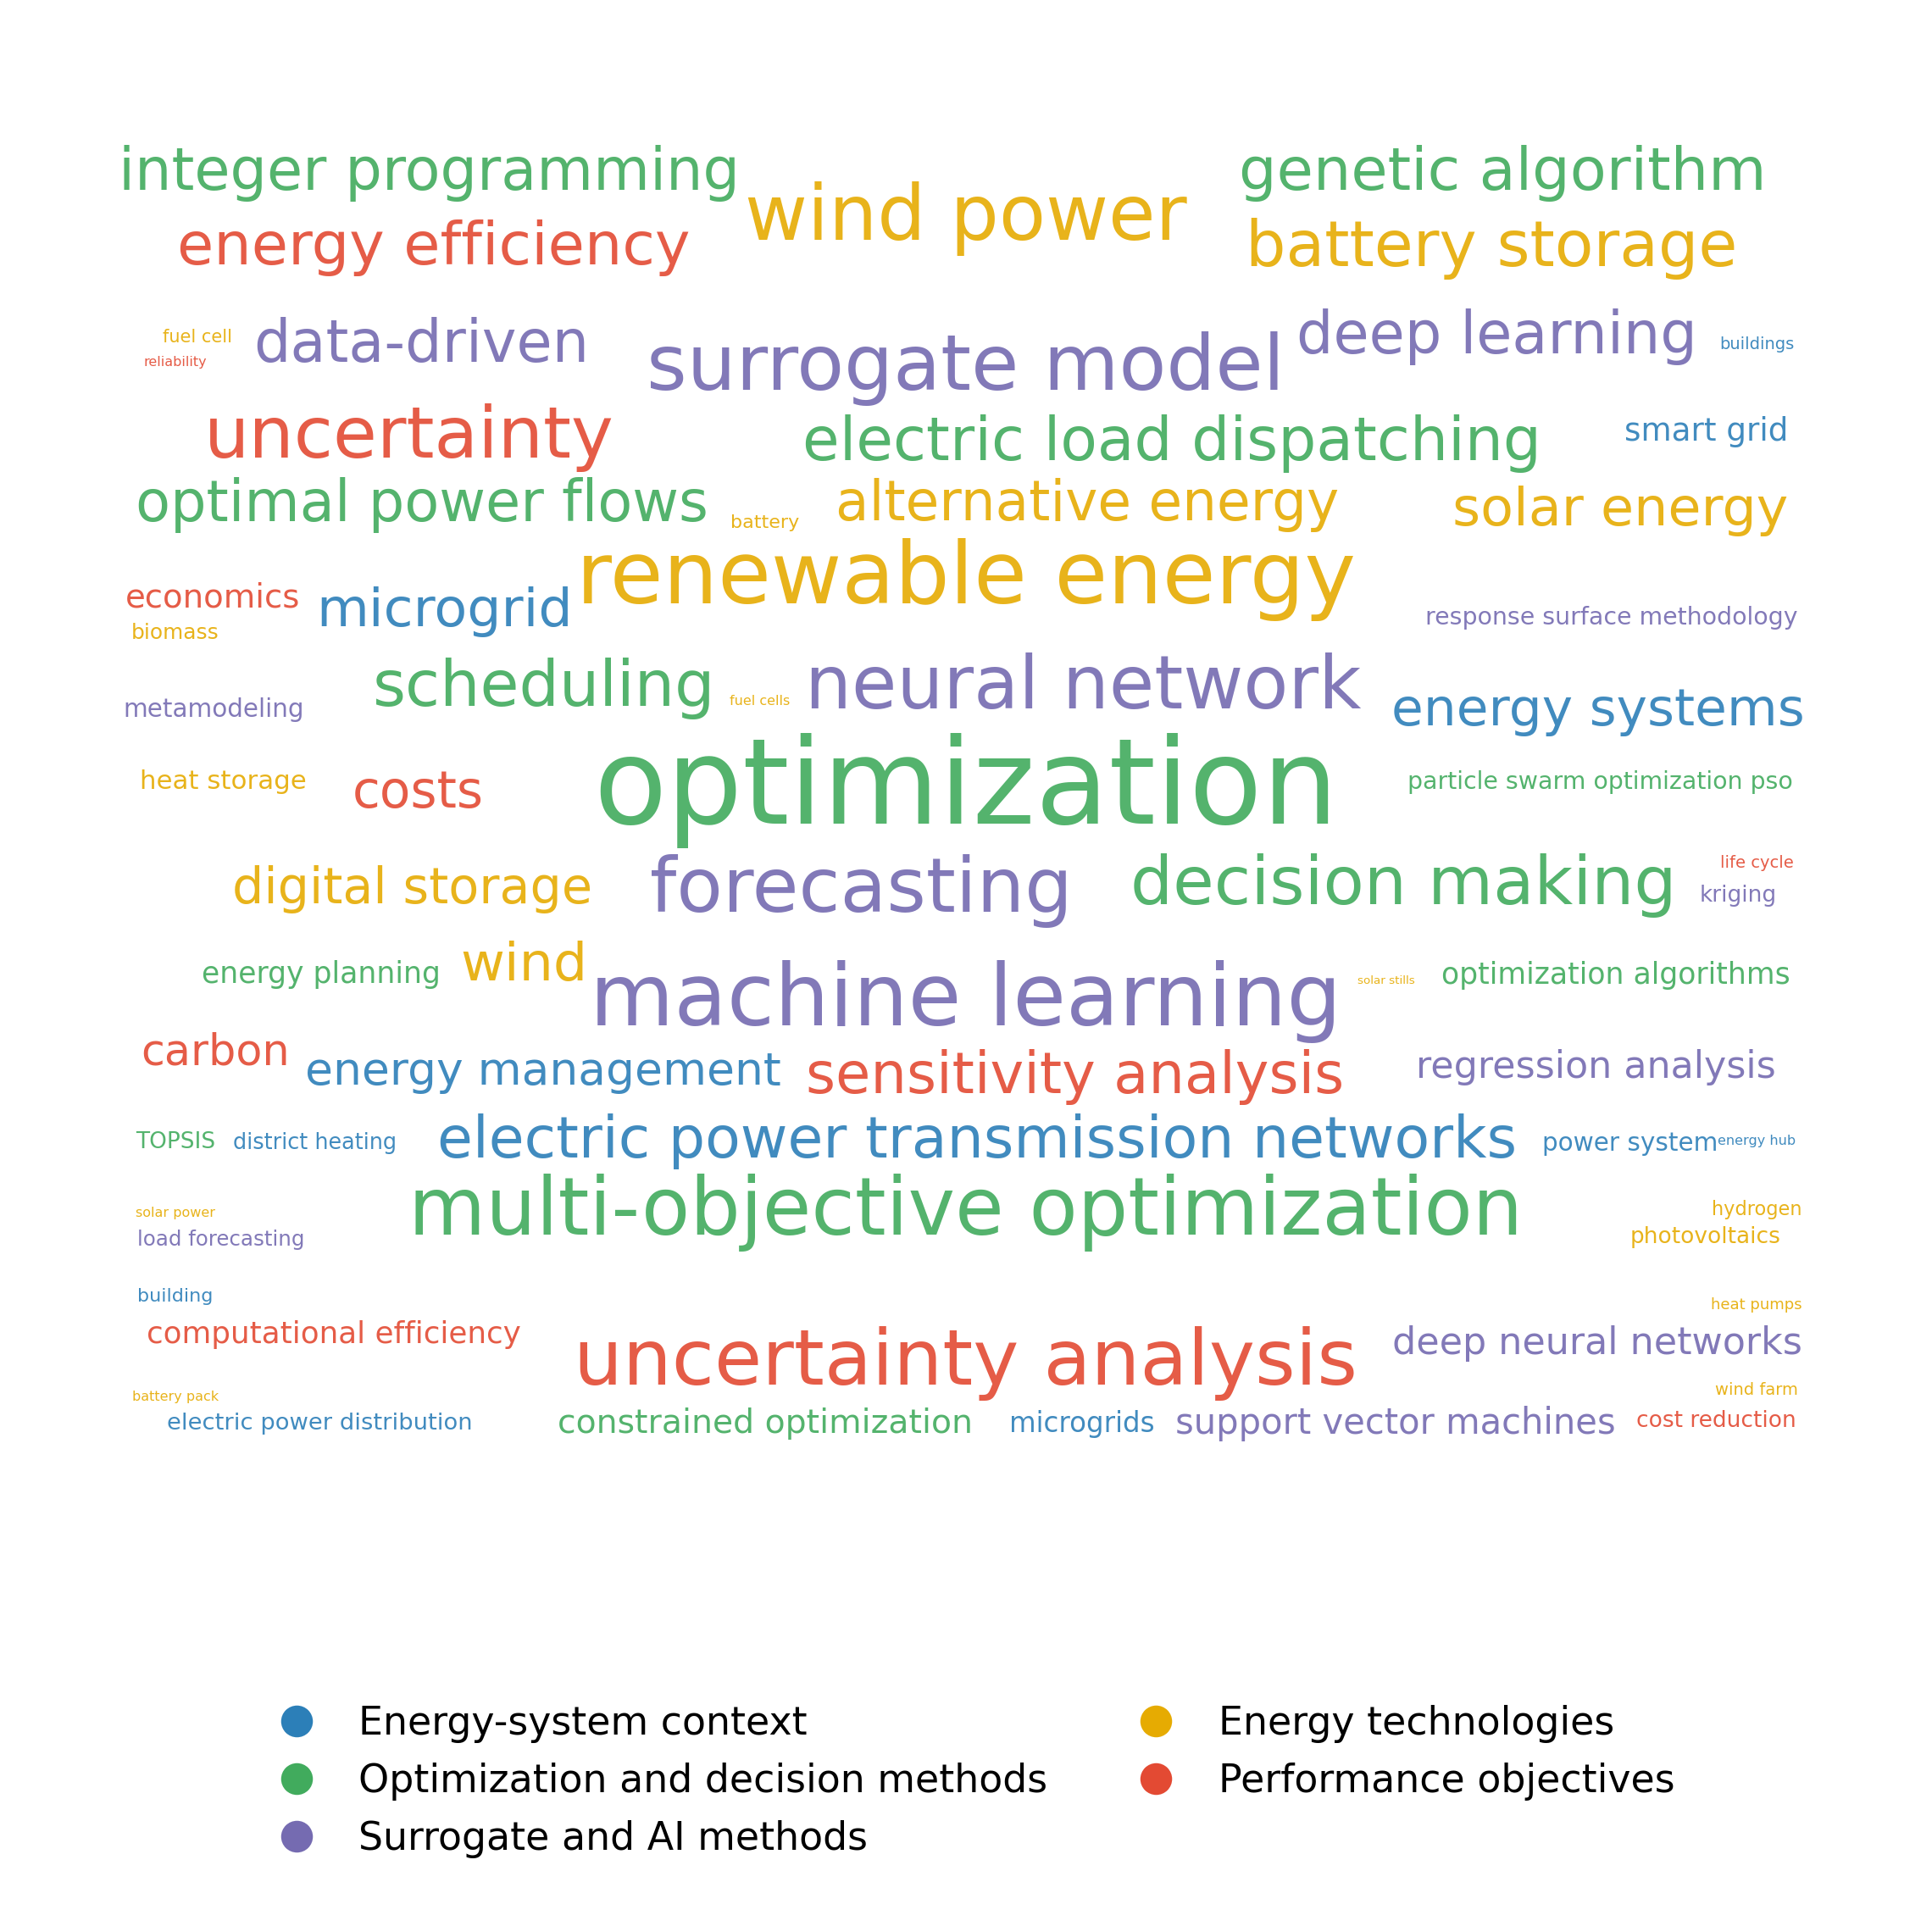
\includegraphics[width=0.98\\linewidth]{../figures/fig_bibliometric_keyword_wordcloud.png}
\caption{Keywords}
\label{fig1}
\end{figure}

For each exported citation record, title, abstract and keywords were
merged into a single text field and classified using a rule-based
screening process. Records were included when explicitly containing
surrogate or metamodel vocabulary, such as surrogate, metamodel,
kriging, Gaussian process, polynomial chaos, response surface or
learning to optimize, with a clear reference to energy systems. These
records were accepted as core literature on surrogate modeling in
optimization-related energy system modeling (n = 1270).

Records which did not contain the explicit surrogate/metamodel
vocabulary mentioned above but showed (i) machine-learning or regression
methodology, (ii) an optimization focus, (iii) an energy-system focus,
and (iv) at least one reference to replacement, approximation or
computation-time reduction compared to an expensive original model were
marked for manual review before included in the main body of analyzed
records (n = 154). A small additional subset (n = 4) was marked as
likely out of scope, because strong non-target signals, such as pure
error diagnosis or site selection without an optimization surrogate. All
remaining records were classified as out of scope (n = 1701), because
they did not meet the surrogate-for-optimization criteria for further
analysis.

To ensure that the review did not only capture explicitly labelled
surrogate studies, the surrogate-focused export was complemented with
MOO/MES studies, comprising records with a multi-objective or
multicriteria focus and a multi-energy or related system context (n =
1674). Together with the surrogate records, this resulted in 2944
bibliographic records before deduplication. DOI- and key-based
deduplication removed 38 duplicates, yielding a database of 2906
records.

For the manuscript, a subset of 285 studies was selected for further
in-depth analysis. These studies thematically match the narrowed
research focus on surrogate modeling, multi-objectivity, and
multi-energy systems. Moreover, 32 previous reviews or overview articles
including bibliometric reviews, were included in a meta-review based on
title, abstract and keywords and compared with the present article.

\section{Bibliometrical analysis}

Figure \ref{bibliometrical} illustrates the bibliometrical analysis
conducted in this review, where a) demonstrates the evolution of journal
articles, conference papers, reviews, conference reviews and book
chapters, b) shows the share of journals, c) the world map of countries
with the highest number of articles, and d) the journals with the most
papers in that field. It can be observed that the number of papers is
growing fast, with the majority being published in Elsevier journals -
mostly \"Applied Energy\", \"Energy\", and \"Energy Conversion and
Management\". China is by far the leading country (896 papers), followed
by Iran (192), India (152), and the USA (145).

\begin{figure*}[t!]
\centering
\includegraphics[width=\textwidth]{./multienergysystems.png}
\caption{Conceptual graph on a multi-energy system}
\label{fig:multienergysystem}
\end{figure*}

\section{Conceptual foundations: multi-energy systems, surrogate models and optimization bottlenecks}

\subsection{Multi-energy systems}

The analysis of MES becomes increasingly important in energy system
modeling due to the ongoing electrification of the heating, transport,
and industry sectors, the shift towards decentralized energy production,
and the intermittent nature of renewable energy systems (RES) that
requires substantial investments in storage capacities and grid
extension. Although a clear definition of MES is absent, MES can be
understood as an extension of hybrid renewable energy systems (HRES),
where HRES usually denote systems combining two or more renewable
generation and storage technologies for reliable renewable electricity
supply, such as PV, Wind, and battery storage, while MES broaden this
scope to coupled electricity, heating, cooling, industry and transport
sectors through centralized and decentralized generation, storage and
conversion technologies, as illustrated in Figure
\ref{fig:multienergysystem}. This cross-sectoral assessment is
crucial owing to the ongoing electrification of the transport and
heating sectors and the intermittency challenge of renewable energy that
necessitates the provision of system flexibilities of a resilient,
cost-efficient, and decarbonized energy system.

While the definition of MES and integrated energy systems (IES) is often
used synonomously, MES refers to the technical modeling of sector
coupling (electricity, heating, transport, industry) and physical energy
flows between sectors. IES, on the other hand, encompass not only the
physical modeling but also regulatory and systemic operational
integration of energy sectors, infrastructures, and markets with the aim
of coordinated planning and operation of all RES and infrastructures.
MES builds thus the physical basis of IES which is the overarching
systemic concept for planning of including grid expansion, market
integration, and energy policies.

Coupling electricity to heat, gas, hydrogen, transport and industrial
processes in optimization models increases both the number of variables
and the number of non-linear relationships, and creates computationally
expensive problems for which surrogates are increasingly used.
\cite{Zhou20181,Zheng20231907,Ren2024,Jalving2023,Dong2023,Yin2024,Cao2023,Wang2020202933}.

\subsection{Surrogate models}

\begin{figure*}[!t]
\centering
\includegraphics[width=\textwidth]{./Surrogate_classification.png}
\caption{Conceptual positioning and classification of surrogate models in energy-system optimization. The figure illustrates how surrogate models mainly act as predictive approximations of expensive energy-system models, but acquire a prescriptive role when embedded in optimization workflows. The lower panel summarizes the four classification axes used in this review: model family, surrogate target, optimizer role and trust mechanism.}
\label{fig:surrogate-classification}
\end{figure*}

Surrogate models, also referred to as metamodels or emulators, are
computationally cheap approximations of an expensive original model.
They are constructed from input--output evaluations of the original
model and are then used to replace, approximate or support selected
parts of an analysis or optimization workflow
\cite{Bhosekar2018,Westermann2019,FernandezGodino2023}. In energy system
optimization, the expensive original model may be a detailed building
simulation, MES optimization, an optimal-power-flow formulation, a
mixed-integer dispatch model, or another high-fidelity numerical model
\cite{Westermann2019,Hirvonen2017323,Manco2024,Klemm2021,Ruan2021221}.
The purpose of the surrogate is therefore not to replace the physical or
optimization model, but to reduce the number, duration or complexity of
expensive model evaluations during design, operation, uncertainty
analysis or multi-objective search
\cite{Bhosekar2018,DiazManriquez2016,Hirvonen2017323}.

In the basic workflow, a set of representative system configurations is
sampled at first. Second, the original model is evaluated for these
configurations, producing training data. Third, a statistical or
machine-learning model is fitted to approximate the mapping from inputs
to outputs based on the generated training data. Once validated, the
surrogate can be evaluated much faster than the original model and can
therefore be used for repeated evaluations inside optimization,
sensitivity or uncertainty analysis
\cite{Bhosekar2018,Westermann2019,FernandezGodino2023}. In building
applications, for example, detailed simulation models, e.g. TRNSYS or
EnergyPlus, are used to generate training samples, while surrogate
models are then used to accelerate optimization
\cite{Hirvonen2017323,Westermann2019,Elwy2024,Zhang2026_building}. In
the solar-community study by Hirvonen et al., a neural network-based
surrogate model is updated iteratively during multi-objective
optimization where candidate solutions are predicted by the surrogate
and re-evaluated in the full TRNSYS model and subsequently added to the
training set \cite{Hirvonen2017323}. Surrogate modeling can either be an
offline approximation step or a part of the optimization loop itself
(in-loop).

\subsection{Optimization problem classes and computational bottlenecks}
\label{sec:optimization-bottlenecks}

Surrogate models become relevant where energy-system optimization
problems are repeatedly solved, computationally expensive, or physically
too detailed to be evaluated multiple times inside a search loop at high
spatio-temporal resolution. The relevant problem classes include
short-term dispatch and unit commitment, optimal power flow, capacity
and generation expansion, district-heating and MES design, stochastic or
robust planning considering uncertainty, and highly constrained
multi-objective optimization
\cite{Wu2022231,Chen20244723,Chen2022,Muhlpfordt20194806,Deng2020831,Khaloie2025,Rodgers2018951,Han2018622,Hirvonen2017323,Zhou20181}.

The computational burden arises from several sources: Dispatch and
models become difficult because of intertemporal storage constraints,
binary on/off decisions, and start-up costs of dispatchable sources.
Moreover, network-constrained problems such as AC OPF add nonlinear
voltage, reactive-power and security constraints require further
computational resources. Capacity-expansion, microgrid-sizing and
MES-design problems are expensive because each candidate solution
usually requires multiple dispatch evaluations. Sector coupling in MES
increases problem size through electricity-heat-gas-hydrogen conversion
technologies, storage State-of-charge (SoC) states and nonlinear
relationships
\cite{Safta20172535,Pang2023,Su2022315,Chen2023657,Koirala20242284,Zheng20231907,Ren2024,Jalving2023,Dong2023,Yin2024}.

Additionally, if uncertainty is considered, stochastic
chance-constrained formulations add scenarios, recourse decisions or
probabilistic constraints, while MOO problem create outer loops in which
multiple candidate solutions must be evaluated to approximate Pareto
fronts
\cite{Hu2020,Hu2021671,Volodina2022,Liang20246508,Thrampoulidis2021,Hussien20211883,Schulte2020,Han2018622}.

\section{A taxonomy of surrogate models for energy system optimization: Model class, surrogate target, integration depth, and trust mechanism}
\label{sec:taxonomy}

FigureÂ~\ref{fig:surrogate-classification} illustrates the conceptual
role and classification scheme of surrogate models in energy system
optimization. It shows that their common application lies between
predictive modeling and optimization-based decision support. Surrogate
models can be classified by 1) model class, 2) surrogate target, 3)
optimizer role, 4) and trust mechanism. These four dimensions separate
the main questions that determine how a surrogate is used in an
optimization model: what mathematical approximation is employed, what
part of the original model is approximated, where the surrogate is
integrated in the optimization, and why its predictions can be trusted
for decision-making.

We propose this taxonomy because model class as the sole distinguishing
feature of surrogate models is not sufficient, because the same model
class can be employed for different purposes in an optimization model. A
Gaussian-process model may approximate an objective function, support
Bayesian infill sampling, quantify prediction uncertainty, or screen
candidate solutions before an expensive simulation is evaluated
\cite{Hu2020,Hu2021671,Volodina2022,Schulte2020}.
Similarly, a neural network may predict demand or renewable generation,
approximate a detailed building simulation or power-flow states, or
directly predict a near-optimal solution
\cite{Ruan2021221,Khaloie2025,Lim2025,Wu2022231,Chen2022,Chen20244723,Li202359995}.

\begin{table*}[!t]
\centering
\scriptsize
\begin{tabularx}{\textwidth}{@{}L{0.16\textwidth} C{0.05\textwidth} C{0.08\textwidth} L{0.21\textwidth} L{0.20\textwidth} L{0.22@\textwidth} Family & Output & Opt. compat. &@{}}
\toprule
Strengths & Typical failure modes & Where it dominates (refs.)
\\
Polynomial RSM / PCE & $p$,$i$ & $\nabla$ $\circ$ $\square$ &
Closed-form moments; analytic chance constraints; parsimonious & Curse
of dimensionality; smoothness assumption; sparse-grid cost &
Chance-constrained AC OPF, stochastic dispatch
\cite{Muhlpfordt20194806,Muhlpfordt20174490,Koirala20242284,Xu20212696,Engelmann20186188}
\\
Kriging / Gaussian process & $p$,$i$ & $\nabla$ & Predictive posterior;
Bayesian acquisition; small-sample use & $O(n^3)$ scaling;
stationarity assumption; kernel choice sensitive & Bayesian optimization
and uncertainty propagation
\cite{Nikolaidis2021,Hu2020,Hu2021671,Volodina2022,Schulte2020,Liu20222679}
\\
Radial basis functions & $p$ & $\nabla$ & Smooth interpolant; cheap;
metaheuristic-friendly & Centre placement is heuristic; weak in
extrapolation & Surrogate-assisted evolutionary OPF and HRES sizing
\cite{Liu20223726,Mahapatra2022721,Mahapatra20161921,Hussien20211883}
\\
Random forest / GBDT & $p$,$i$ & $\square$ & Mixed inputs; fast
classification and regression; quantile variants & Step responses break
gradients; piecewise-constant tails & Unit-status identification,
chance-constraint surrogates and thermal-interference screening
\cite{Liang20246508,Chen2023657,Petrova2025}
\\
Neural networks (MLP / CNN / RNN) & $p$ & $\nabla$ ($\square$) &
Universal approximation; large-data scaling; transfer learning &
Black-box; calibration drift; overconfidence on OOD & End-to-end OPF,
demand and price forecasting
\cite{Chen20244723,Chen2022,Wu2022231,Xu20223066,Guo20222057,Li202359995}
\\
Hard-constrained / structure-preserving NN & $p$ & $\nabla$ $\circ$
$\square$ & Encodes feasibility or structural constraints; can support
exact reformulation & Constraint design is problem-specific; training
and reformulation can be costly & Feasible dispatch proxies and
MILP-embedded conversion-loss surrogates
\cite{Chen20244723,Li202359995,Liu20242534}
\\
Graph neural networks & $p$ & $\nabla$ & Topology-aware; transferable
across grid sizes & Message-passing depth; oversmoothing on radial
grid trees & Wind-farm and multi-fidelity power-flow surrogates
\cite{Park2019,Taghizadeh2024,Khayambashi202453}
\\
Decision-focused / L2O proxies & $p$ & $\nabla$ & Trained for decision
quality, not regression error & Feasibility restoration needed; dataset
is optimizer-synthetic & Learning-to-optimize for SCED / SCUC / OPF
\cite{Wu2022231,Chen20244723,Chen2022,Li2023__2,Wu2024391,Liang20246508}
\\
\end{tabularx}
\end{table*}

\subsection{Model classes}
\label{sec:surrogate_classes}

TableÂ~\ref{tab:T1-taxonomy} compiles the most commong model classes in
the reviewed literature, the type of output they produce (point or
interval/posterior), their compatibility with the dominant optimizer
classes (gradient-based, convex, mixed-integer), and their typical
failure modes.

\subsubsection{Polynomial response surfaces and polynomial chaos expansions}
\label{sec:tax:rsm}

\paragraph{Polynomial response surface}

A polynomial response surface is a simple surrogate model that
approximates the relationship between design variables and a result
using a polynomial. Instead of running an expensive simulation or
optimization for each new combination of design variables, one can
estimate a function like:

$$\begin{equation}
 y \approx \beta_0 + \sum_{i=1}^{n} \beta_i x_i + \sum_{i=1}^{n} \beta_{ii} x_i^2 + \sum_{i<j}^{n} \beta_{ij} x_i x_j
\end{equation}$$

where $y$ denotes an output of interest, such as costs, CO~2~ emissions,
or efficiency, while $x_i$ represents the $i$-th design variable, such
as PV capacity, battery capacity, or electrolyzer power. The
coefficients $\beta$ are estimated from previously evaluated training
data.

Response-surface methodology (RSM) has been applied in PV control
parameter tuning \cite{Hasanien2018168}, thermal-system optimization
problems \cite{Sami20181416,Ahmad202451,Sun2020}, in chance-constrained
AC optimal power flow as an iterative response-surface refinement
\cite{Xu20212696}, and in green-hydrogen production models
\cite{Ahmad202451}.

Polynomial response surfaces have the advantage of clear
interpretability, ease of fit on small designs and direct compatibility
with gradient-based and convex solvers. A limitation is the curse of
dimensionality: the number of polynomial terms grows rapidly with the
number of inputs and polynomial order, while low-order response surfaces
may miss strong nonlinearities and interactions
\cite{Torun20192128,Hasanien2018168}.

\paragraph{Polynomial chaos expansion}

Polynomial chaos expansions (PCE) extend response surface methods to a
probabilistic approach by representing the model output as an expansion
in orthogonal polynomial basis functions of random input variables. For
example, considering the optimization of a PV--BESS--H$_2$ system, where
the output $Y$ denote annual system costs, CO~2~ emissions, or grid
imports, these outputs depend on uncertain input variables such as
electricity prices or load profiles. A polynomial chaos expansion
approximates the expensive optimization model as a function of these
uncertain inputs:

$$\begin{equation}
 Y \approx \sum_{\alpha \in \mathcal{A}} c_{\alpha} \Psi_{\alpha}(\boldsymbol{\xi})
\end{equation}$$ $$\begin{equation}
 \boldsymbol{\xi} = \left[ \xi_{\mathrm{price}}, \xi_{\mathrm{PV}}, \xi_{\mathrm{load}}, \xi_{\mathrm{H_2}}, \xi_{\mathrm{CAPEX}} \right].
\end{equation}$$

where, $Y$ denotes the model output, $\boldsymbol{\xi}$ is the vector of
random input variables, $\Psi_{\alpha}$ are multivariate orthogonal
polynomial basis functions, and $c_{\alpha}$ are expansion coefficients
estimated from model evaluations.

Mühlpfordt et al.Â~\cite{Muhlpfordt20194806} introduced the
chance-constrained AC optimal power flow using PCE and recent work
employed general PCE-based hosting-capacity calculations
\cite{Koirala20242284}, to data-driven distribution planning
\cite{Fu20202904,Fu2022}, and to uncertainty quantification in stochastic
economic dispatch \cite{Safta20172535}.

Because the expansion coefficients provide direct access to output
statistics, such as the mean and variance, without requiring additional
Monte Carlo sampling, PCE is particularly beneficial for uncertainty
propagation such as chance-constrained optimization AC optimal power
flow, hosting-capacity analysis and stochastic dispatch
\cite{Muhlpfordt20194806,Safta20172535,Xu20212696,Koirala20242284}.
Thus, PCE provide simple and interpretable approximations for design and
process optimization
\cite{Hasanien2018168,Sami20181416,Ahmad202451}.
However, the limitation is the rapid growth of the polynomial basis with
the number of stochastic input dimensions and by reduced accuracy for
non-smooth model responses
\cite{Muhlpfordt20194806,Safta20172535,Koirala20242284,Xu20212696}.

\subsubsection{Gaussian process regression and kriging}
\label{sec:tax:gp}

Gaussian process (GP) regression, also known as kriging in
geostatistics, is a widely established surrogate modeling approach for
optimization and Bayesian uncertainty quantification. Kriging originally
referred to optimal spatial interpolation based on a covariance
structure, whereas GP regression formulates the same idea in a
probabilistic machine-learning framework. In surrogate modeling, both
terms are commonly used for probabilistic surrogate models that provide
not only a point prediction, but also an associated predictive
uncertainty.

In an energy-system optimization problem, the input vector $\mathbf{x}$
may contain design variables such as PV capacity, battery capacity,
electrolyzer power, hydrogen storage capacity, and fuel-cell power:

$$\begin{equation}
 \mathbf{x} = \left[ P_{\mathrm{PV}}, E_{\mathrm{BESS}}, P_{\mathrm{ELY}}, E_{\mathrm{H_2}}, P_{\mathrm{FC}} \right].
\end{equation}$$

The corresponding model output $y$ may denote annual system costs, CO~2~
emissions, grid imports, or another performance indicator obtained from
a detailed optimization model. A key advantage of GP regression is that
it predicts both the expected system performance and the uncertainty of
this prediction:

$$\begin{equation}
 \hat{y}(\mathbf{x}) = \mu(\mathbf{x}) \pm \sigma(\mathbf{x}).
\end{equation}$$

Here, $\hat{y}(\mathbf{x})$ denotes the surrogate prediction for a given
energy-system design, $\mu(\mathbf{x})$ is the predicted mean
performance, and $\sigma(\mathbf{x})$ represents the predictive
uncertainty. In practical terms, the mean prediction indicates how
promising a design is, while the uncertainty estimate indicates how
confident the surrogate is in this prediction.

In dispatch and operations, Nikolaidis et al.Â~\cite{Nikolaidis2021} used
GP-based Bayesian optimization, demonstrating substantial reductions in
the number of MILP evaluations. Hu et al.Â~\cite{Hu2020,Hu2021671} use GP
regression to propagate uncertainty in stochastic economic dispatch,
with a Bayesian-network extension in \cite{Volodina2022}. Wang et
al.Â~\cite{Wang2023} employ GP regression in an LSTM-based hybrid for
wind-power forecasting and dispatch, similar to that used by Zhang et
al.Â~\cite{Zhang2019270}. In Bayesian power-network planning \cite{Lawson201647}
GPs often serve as a surrogate model for transmission expansion under
uncertainty. In design and capacity expansion optimization studies,
kriging-based surrogate modeling has been used to solve large optimal
power flows \cite{Deng2020831} and to optimize battery thermal management
with GP-based screening \cite{Li2021,Babaeiyazdi2021,Kong2021}.
GP and kriging models are also used in surrogate-assisted design search
and calibration, including geothermal design, building and HVAC
calibration, and interactive multi-objective building-energy design
\cite{Schulte2020,Chakrabarty2021,Aghaei Pour2022303}.

A major limitation of GP regression is its computational cost. Standard
GP training becomes increasingly expensive as the number of evaluated
simulation points grows, because the model has to account for the
correlation between all training data points, making it difficult to
apply to very large training data sets. This problem can be addressed by
reducing the amount of data or correlation structure that the GP has to
process. For example, sparse kernel methods simplify the covariance
structure by assuming that only the most relevant or nearby training
points have a strong influence on a prediction. Moreover, local GP
models can be used to split the design space into smaller regions and
fit separate Gaussian processes within these regions, so that each model
only uses a subset of the full training data. Inducing-point methods
replace the full training set with a smaller set of representative
support points, which summarize the main structure of the data. These
approaches make GP regression more scalable when the number of runs
grows, but they are also accompanied by a loss of approximation
accuracy \cite{Hu2020,Volodina2022,Liu20222679}.

\subsubsection{Radial-basis-function networks and kernel regressors}
\label{sec:tax:rbf}

Radial-basis-function (RBF) models are deterministic surrogate models
that combine several localized basis functions (functions that have a
strong effect in a specific area of the input/design space and less in
another). The basic idea is that a new design is predicted from its
similarity to previously selected support points. Designs close to a
support point have a strong influence on the prediction, while distant
designs have only a weak influence. An RBF surrogate approximates this
output as a weighted sum of radial basis functions:

$$\begin{equation}
 \hat{y}(\mathbf{x}) = \sum_{j=1}^{M} w_j \, \phi\left(\left\| \mathbf{x} - \mathbf{c}_j \right\|\right).
\end{equation}$$

Here, $\mathbf{c}_j$ denotes the $j$-th support point, $w_j$ is its
fitted weight, and $\phi(\cdot)$ is a radial basis function that depends
on the distance between the new design $\mathbf{x}$ and the support
point $\mathbf{c}_j$.

A common choice is the Gaussian radial basis function:

$$\begin{equation}
 \phi\left(\left\| \mathbf{x} - \mathbf{c}_j \right\|\right) = \exp\left( -\frac{\left\| \mathbf{x} - \mathbf{c}_j \right\|^2}{2\sigma^2} \right).
\end{equation}$$

This means that nearby energy-system designs have a stronger effect on
the prediction than distant designs. Compared with Gaussian process
regression, RBF models use a similar distance-based function, but they
usually provide a deterministic prediction rather than a full posterior
uncertainty distribution. This makes them computationally less expensive
when the surrogate has to be evaluated many times, for example during
candidate sampling.

Urgun et al.Â~\cite{Urgun20202791} use multilabel RBF classification for
importance-sampled composite-power-system reliability, and
Karamichailidou et al.Â~\cite{Karamichailidou20212137} use RBF to model
wind-turbine power curves for economic dispatch. RBF is also used in PV
production \cite{Yang2020415,Tian2020}, and have been used as the
regression back-end in extreme-learning-machine load forecasting
\cite{Zeng2017175,Sideratos2020,Madhukumar20228891,Rafi202132436}. In
building-energy applications, SVR and ANN metamodels have been used to
predict district cooling loads \cite{Jia2022553}, while an ANN trained on
EnergyPlus simulations has supplied fitness values to a genetic
algorithm for heating set-point scheduling \cite{Reynolds2017704}.

RBF models show fast evaluation and work well with relatively small
training data sets. However, their predictions are only reliable within
the region covered by the evaluated simulation points. For new
energy-system designs that are far away from the training data, e.g.
very different combinations of PV capacity, battery capacity,
electrolyzer power, or hydrogen storage size, RBF models show rather
poor approximation. Therefore, RBF-based optimization is often combined
with active-sampling strategies to add new simulations in promising or
poorly covered parts of the design space.
\cite{Deng2020831,Tian2020,Han2018622,Pang2023}.

\subsubsection{Tree ensembles: random forests and gradient boosting}
\label{sec:tax:trees}

Tree ensembles combine decision trees to obtain more accurate
predictions than a single tree. They are widely used for regression and
classification tasks in energy-system optimization models for different
tasks because due to their ability to perform well on structured tabular
data and can capture nonlinear relationships and interactions between
input variables. In tree-ensembles, the output is a continuous
performance indicator, such as costs or CO~2~ emissions. In
classification tasks, the output is a discrete class label, for example
whether an energy-system design is feasible or infeasible.

For a random forest, the prediction is obtained by averaging the outputs
of many individual decision trees:

$$\begin{equation}
 \hat{y}(\mathbf{x}) = \frac{1}{B} \sum_{b=1}^{B} T_b(\mathbf{x}),
\end{equation}$$

where $T_b(\mathbf{x})$ is the prediction of the $b$-th tree and $B$ is
the number of trees in the ensemble. In classification tasks, such as
predicting whether an operating point infeasible, the individual trees
vote for a class instead of returning a continuous value.

Gradient-boosted trees use a different principle: Instead of training
all trees independently, they build the ensemble sequentially where each
new tree is trained to correct the remaining error of the previous
trees:

$$\begin{equation}
 \hat{y}(\mathbf{x}) = \sum_{m=1}^{M} \eta_m T_m(\mathbf{x}),
\end{equation}$$

where $T_m(\mathbf{x})$ denotes the $m$-th tree and $\eta_m$ is its
learning weight. XGBoost is a widely used implementation of this
gradient-boosting principle. Tree-based ensemble methods have been used
in microgrid scheduling to serve as fast predictive models that
approximate the performance or feasibility of candidate operating
schedules, thereby reducing the number of detailed simulation or
optimization runs required,
\cite{Eseye201991463,Faraji2020157284,Wang20192635,Nematollahi2021},
distribution-system planning under uncertainty
\cite{Fu20202904,Fu2022,Jahangiri20244849,Jahangiri2023}, and
short-term wind, solar and load forecasting that determines optimization
dispatch \cite{Li2020,Hanifi2024,Alkesaiberi2022,Madhukumar20228891}.
Also, tree ensembles have been used in surrogate-assisted MOO where they
classify candidate decisions as feasible or infeasible before more
expensive optimization
\cite{Han2018622,Schulte2020,Pang2023,Xiao2018}.

The main advantage of tree ensembles is that they can model complex
nonlinear effects without requiring an explicit functional form. For
example, they can learn how the effect of battery capacity depends on PV
capacity, electricity prices, or hydrogen storage size. A limitation of
tree-based models is, however, that their predictions are
piecewise-constant or piecewise-linear and therefore do not provide
smooth gradients. This means that they change their prediction abruptly
at decision boundaries instead of forming a smooth function; therefore,
continuous derivatives, as required by gradient-based optimizers, cannot
be used. This makes them difficult to embed directly into gradient-based
nonlinear programming problems. In practice, tree models are therefore
often used outside the optimization model as fast prediction models, for
example to evaluate candidate solutions before or after
optimization.\cite{Ren2024,Lin2023,Pang2023,Wang20211767}.

\subsubsection{Neural surrogates: MLP, recurrent and graph architectures}
\label{sec:tax:nn}

Neural networks are widely used as surrogate models in recent
energy-system literature because they can approximate complex nonlinear
relationships between inputs and outputs. In contrast to simpler
surrogate models, neural networks can learn interactions between many
design variables, operating conditions, and time-dependent system
states. This makes them especially beneficial for highly complex
nonlinear optimization models.

A neural network-based surrogate learns an approximate relationship from
inputs to outputs:

$$\begin{equation}
 \hat{y} = f_{\theta}(\mathbf{x}),
\end{equation}$$

where $f_{\theta}$ denotes the neural network and $\theta$ represents
its trained weights.

For static design problems, multilayer perceptrons (MLPs) are commonly
used. They relate a fixed input vector, such as technology capacities
and cost assumptions, to one or more performance indicators:

$$\begin{equation}
 \hat{y} = f_{\theta} \left( P_{\mathrm{PV}}, E_{\mathrm{BESS}}, P_{\mathrm{ELY}}, E_{\mathrm{H_2}}, P_{\mathrm{FC}} \right).
\end{equation}$$

For time-dependent problems, recurrent neural networks can be used to
learn from input trajectories, such as hourly demand, renewable
generation, prices, or storage states:

$$\begin{equation}
 \hat{y}_t = f_{\theta} \left( \mathbf{x}_1,\mathbf{x}_2,\ldots,\mathbf{x}_t \right).
\end{equation}$$

This is useful when the surrogate has to approximate dispatch behaviour,
storage operation, or system states over time. Graph neural networks are
particularly relevant for networked energy systems because they can
represent the physical structure of electricity, gas, or heat networks.
In this case, buses, substations, buildings, or heat network nodes are
represented as graph nodes, while power lines, pipes, or thermal
connections are represented as edges. A graph-based surrogate can
therefore learn how local injections, loads, or temperatures evolve
throughout the network:

$$\begin{equation}
 \hat{\mathbf{y}} = f_{\theta} \left( \mathbf{X}, \mathbf{A} \right),
\end{equation}$$

where $\mathbf{X}$ contains node-level features such as demand,
generation, temperature, or pressure, and $\mathbf{A}$ describes the
network topology.

MLPs are used when the surrogate receives a fixed-size input vector and
returns a fixed-size output vector. This is typical for optimization
problems in which variables such as technology capacities, demand
levels, or prices are used to predict performance indicators (e.g. costs
or emissions). Because trained MLPs are fast to evaluate, they are
useful when many candidate solutions have to be assessed during an
optimization.

In the reviewed literature, MLPs have been used as fast approximations
of costs, feasibility, or security constraints in security-constrained
economic dispatch
\cite{Chen2022,Chen20244723,Wu2022231,Xu20223066,Guo20222057,Li202359995}.
They are also used in response-surface models in metamodel-based design
search, where they replace repeated evaluations of more detailed
optimization models
\cite{Hirvonen2017323,Jia2022553,Li2023,Wang2020202933}.
In the building sector, MLPs are used as surrogates for retrofit
analysis, for example to approximate energy demand, costs, or other
building-performance indicators
\cite{Thrampoulidis2021,Reynolds2017704,Koschwitz2018134}. Recurrent and
convolutional neural networks are used when the input is sequential
rather than static, meaning that the surrogate has to learn from ordered
time-series data, such as hourly demand, renewable generation,
electricity prices, or storage states. This includes long short-term
memory (LSTM) networks, gated recurrent units (GRUs), convolutional
neural networks (CNNs), and hybrid convolutional neural network--long
short-term memory (CNN--LSTM) models. They are widely used in dispatch
and storage scheduling, where current decisions depend on previous
system states and operating conditions
\cite{Rafi202132436,Sideratos2020,Li2019,Tian2020,Yang2020415,Wang2023,Shi2024,Lu20232989,Hanifi2024}.
Graph neural networks (GNNs) are increasingly used for network-based
energy-system optimization problems. They are well suited to analyze
power flows, voltage magnitudes because they can use the topology of the
underlying grid directly. In this representation, buses, substations, or
other network nodes are treated as graph nodes, while lines or pipes are
represented as graph edges
\cite{Park2019,Su2022315,Liu20223726,Chen2023657}. Where the
underlying physical equations are well understood, physics-informed
neural networks (PINNs) can include these equations directly in the
training data. This can reduce extrapolation error, because the
surrogate is not only fitted to data but also encouraged to respect
known physical constraints
\cite{Park2019,Su2022315,Liu20222679,Chen2023657}.

Overall, neural surrogates can represent nonlinear, temporal, and
especially network-dependent system behaviour. Their main limitations
are the need for sufficient training data, weaker interpretability
compared with simpler models, and the risk of poor generalization
outside the range of the training data.

\subsection{Surrogate targets}
\label{sec:tax:targets}

Surrogate models can also be classified by their target, i.e. what the
surrogate approximates. Some surrogates approximate exogenous inputs
such as load, weather, renewable energy generation or prices, which
serve as an input to the optimization model
\cite{Eseye201991463,Li2020,Hanifi2024,Conti2026}. Objective values
can be approximated directly, such as energy demand, cost, or emissions
\cite{Westermann2019,Hirvonen2017323,Ahmad202451}, or
physical states or constraints, such as voltage magnitudes, line flows,
storage states, indoor temperatures, thermal-network states or
feasibility violations can be emulated
\cite{Park2019,Su2022315,Mohammadi2024,Khaloie2025}. Surrogates can
also approximate probability distributions, posterior variance,
quantiles or chance-constraint terms
\cite{Muhlpfordt20194806,Hu2020,Volodina2022,Tan2026}, and
learning-to-optimize approaches approximate decisions directly, for
example dispatch vectors, active sets, optimal power flow solutions, or
dispatch schedules
\cite{Wu2022231,Chen2022,Chen20244723,Xu20223066,Li202359995,Liang20246508}.

\subsection{Optimizer integration depth}
\label{sec:tax:integration-depth}

Surrogate models can also be classified according to integration depth
in the optimization.
FigureÂ~\ref{fig:taxonomy-integration-depth} shows how the reviewed
literature is distributed across optimizer integration depth and how it
relates to surrogate target, model class and trust mechanism. In a weak
integration, the surrogate provides forecasts, physical data, or
preprocessed inputs outside of the optimization model itself
\cite{Eseye201991463,Li2020,Hanifi2024}. Surrogates can also preselect
candidate solutions or identify promising regions before expensive model
evaluations are used \cite{Han2018622,Schulte2020,Pang2023,Xiao2018}
or replace a computationally expensive objective function or physical
simulations, and perform constraint checks
\cite{Hirvonen2017323,Deng2020831,Thrampoulidis2021}. In
Bayesian optimization and surrogate-assisted evolutionary algorithm
optimization, surrogate models can balance the exploration of promising
and uncertain search spaces
\cite{DiazManriquez2016,Hu2020,Schulte2020,Volodina2022}. Surrogate
can also be embedded into the optimization problem, for example as a
mixed-integer-compatible approximation
\cite{Wu2022231,Chen2022,Lin2023,Pang2023}. At the strongest
integration depth, learning-to-optimize models replace the optimizer by
predicting decisions directly
\cite{Wu2022231,Chen20244723,Li202359995,Liang20246508}.

\subsection{Trust mechanisms and optimizer-compatible surrogates}
\label{sec:tax:trust-mechanisms}

Another taxonomy dimension is the trust mechanism. Usually, in black-box
surrogate models, which are purely data-driven approximations whose
internal structure is not constrained by physical equations or
optimization constraints, prediction errors on validation data, mostly
Root Mean Squared Error (RMSE), Mean Absolute Error (MAE) or the
coefficient of determination $R^2$ are used to validate the surrogate
model \cite{Westermann2019,Zhang2026_building,Elwy2024}. For many
optimization studies, however, these predictive accuracy metrics alone
are often insufficient: a small average error can still lead to wrong
rankings of candidate solutions, infeasible solutions, or constraint
violations \cite{DiazManriquez2016,Ruan2021221,Khaloie2025,Lim2025}.

Some surrogate classes, therefore, provide additional trust mechanisms.
Gaussian processes and Bayesian models provide posterior uncertainty
that can be used for acquisition functions, which determine the next
optimal evaluation point based on model predictions
\cite{Hu2020,Hu2021671,Tan2026}. Polynomial chaos expansions provide
uncertainty propagation for probabilistic constraints
\cite{Muhlpfordt20194806,Safta20172535,Koirala20242284}, and
physics-informed neural network (PINN) models are validated through
balance equations, physical structure or network topology
\cite{Park2019,Su2022315,Mohammadi2024,Petrova2025,Du2025}. Thus,
decision-focused surrogates should be assessed by their effect on the
optimization results, such as feasibility rate, Pareto-front quality,
and constraint violation in relationship to computational acceleration
\cite{Ruan2021221,Khaloie2025,Lim2025,Chen20244723}.

\subsubsection{Optimization-aware surrogate formulations}
\label{sec:tax:physics-guided}

The preceding subsection classified surrogates mainly by model class.
For optimization, however, the model class alone is often not the most
important property. A surrogate with low prediction error can still lead
to infeasible solutions or distorted Pareto fronts when it is used
inside an optimizer
\cite{DiazManriquez2016,Ruan2021221,Khaloie2025,Lim2025}. Therefore,
some surrogate approaches are better described by how they make the
approximation reliable enough for optimization. In the reviewed
literature, three such optimization-aware surrogate formulations are
particularly relevant: physics-guided modeling, structure-preserving
formulations and decision-oriented surrogates.

\paragraph{Physics-guided and hybrid surrogates}

Physics-guided and hybrid surrogates use available physical knowledge
and information instead of learning the full input-output relation from
data alone. This knowledge may enter the optimization model through
simplified physical equations. The purpose is to improve computational
efficiency and extrapolation, especially when training data are sparse
or when the optimizer evaluates the surrogate outside the original
training range.

A common form is residual learning:

$$\begin{equation}
 \hat{y}(x) = f_{\mathrm{phys}}(x) + r_{\theta}(x),
\end{equation}$$

where $f_{\mathrm{phys}}$ is a simplified physical model and
$r_{\theta}$ is a learned correction term. The physical model captures
the main system behaviour, while the residual model learns the remaining
mismatch. This approach has been used in power-system, multi-energy and
sector-coupled applications where a complete high-fidelity model is too
expensive for repeated use inside the optimizer
\cite{Park2019,Liu20223726,Chen2023657,Liu20222679,Ren2024,Jalving2023,Zheng20231907}.
Physics-informed neural networks are one specific case of this broader
class. Their defining feature is not only the neural-network
architecture, but the inclusion of physical residuals in the training
loss. In energy-system models, such residuals may represent power
balance, heat balance, storage dynamics, network-flow equations or
conversion constraints. Related structure-preserving approaches embed
physical balances or known network structure directly into the
surrogate architecture or optimization layer
\cite{Park2019,Liu20223726,Chen2023657,Liu20242534}.
The main advantage is improved physical plausibility; the main
limitation is that the simplified physics and the residual weights must
be chosen carefully, otherwise the surrogate may become biased or
difficult to train.

\paragraph{Structure-preserving and solver-compatible surrogates}
\label{sec:tax:structured}

Structure-preserving and solver-compatible surrogates are designed so
that the approximation retains properties needed by the optimization
model. These properties may include convexity, monotonicity, feasibility
preservation, active-set consistency or compatibility with mixed-integer
linear formulations. This is especially important when the surrogate
approximates constraints, feasibility regions, cost curves, conversion
losses or operational decisions, because small prediction errors can
directly change the optimal solution. Convex or monotone surrogates are
designed so that they do not only fit the training data, but also
preserve known shape properties of the original model. For example, if
fuel use always increases when output power increases, the surrogate
should also be monotone. If operating costs increase in a convex way
with load or capacity, the surrogate should preserve this convex shape.
Such restrictions make the surrogate less flexible than a fully
black-box model, but they reduce the risk that the optimizer exploits
physically implausible artefacts of the approximation
\cite{Wang2020202933,Hirvonen2017323,Liu20223726,Chen2023657,Chen20244723}.

Other approaches aim at direct solver compatibility. For example,
piecewise-linear neural networks, especially ReLU-based networks (i.e.,
networks using the activation function $\mathrm{ReLU}(z)=\max(0,z)$,
which makes the learned mapping piecewise linear), can in some cases be
reformulated as mixed-integer linear constraints and embedded into a
MILP. This can make the surrogate usable inside an optimization model,
but also increase the model size through additional binary variables and
big-$M$ constraints, i.e. constraints that use a sufficiently large
constant $M$ to switch linear constraints on or off depending on binary
variables.\cite{Wu2022231,Chen2022,Xu20223066,Lin2023}.

A related group of methods enforces hard linear constraints, predicts
active sets, or generates near-feasible solutions that the optimizer can
validate, repair or refine \cite{Chen20244723,Li202359995}. These
surrogates are therefore not only judged by prediction accuracy. They
are useful because they preserve enough of the original optimization
model to avoid poor prediction accuracy. Their main limitation is the
trade-off between structure and flexibility: stronger restrictions can
improve feasibility and solver compatibility, but may reduce
approximation accuracy or make the embedded optimization problem larger.

\subsubsection{Decision-oriented surrogates and learning-to-optimize}
\label{sec:tax:l2o}

Instead of approximating an intermediate model output, decision-oriented
surrogates approximate the solution of an optimization problem, or at
least a solution-related object such as a dispatch vector. In this case,
the surrogate target is no longer only a system response or constraint
term, but the decision itself.

For example, an optimization problem relates data $p$, such as demand,
renewable generation, network state or prices, to an optimal solution:

$$\begin{equation}
 x^{\star}(p) = \arg\min_{x \in \mathcal{X}(p)} f(x,p).
\end{equation}$$

A learning-to-optimize surrogate learns an approximation of this
relation

$$\begin{equation}
 \hat{x}_{\theta}(p) \approx x^{\star}(p),
\end{equation}$$

and can then be used as a direct solution proxy.

This approach is particularly prominent in power-system optimization. Wu
et al.Â~\cite{Wu2022231} train a deep neural network to solve
security-constrained unit commitment with uncertain wind power. Chen et
al.Â~\cite{Chen2022,Chen20244723} learn optimization proxies for
large-scale security-constrained economic dispatch with feasibility
guarantees. Guo et al.Â~\cite{Guo20222057} learn optimal power allocation in
islanded microgrids, and Xu et al.Â~\cite{Xu20223066} train an ensemble deep
network for non-convex economic dispatch. Li et al.Â~\cite{Li202359995} learn
to solve optimization problems with hard linear constraints, while Liang
et al.Â~\cite{Liang20246508} combine learning-to-optimize with statistically
feasible optimization for chance-constrained dispatch.

Recent reviews show the rapid growth of this in power-system modeling
\cite{Khaloie2025,Lim2025,Ruan2021221}. If the surrogate predicts a
feasible or near-feasible solution, the model can avoid solving a large
MILP or dispatch problem from scratch, or can at least start the solver
from a much better initial point. The main risk is that the surrogate
now directly affects the decision. Its validation must therefore go
beyond the basic prediction error metrics such as RSME, MAE, and $R^2$,
and include feasibility rate, constraint violation, and robustness using
sensitivity analysis.

\section{Meta review of surrogate modeling and multi-energy systems}
\label{sec:related-reviews}

TableÂ~\ref{tab:T7-related-reviews} compares prior review studies
identified through our literature selection process.

\begin{table*}[!t]
\centering
\scriptsize
\begin{tabularx}{\textwidth}{@{}@ L{0.015\textwidth} C{0.025\textwidth} L{0.050\textwidth} L{0.150\textwidth} L{0.155\textwidth} L{0.25\textwidth} L{0.30\textwidth} @ Ref. & Year &@{}}
\toprule
Reviewed material & Method scope & Application scope & Main outcome &
Research gaps identified\
\\
\cite{Bhosekar2018} & 2018 & ref. list: 126 & Surrogate modelling,
feasibility analysis, derivative-free optimization; RBF and kriging &
Generic engineering and chemical-engineering optimization & Reviews
surrogate models for modelling, feasibility analysis and optimization;
emphasizes problem-dependent surrogate choice. & Need for better
model-selection guidance and more reliable surrogate use in constrained
expensive optimization.\
\cite{DiazManriquez2016} & 2016 & ref. list: 64 & Surrogate-assisted MOEAs;
fitness replacement; evolution control & Generic expensive
multi-objective optimization & Classifies surrogate-assisted MOEAs by
how the surrogate interacts with the evolutionary search. & Need to
control surrogate error and avoid false Pareto fronts when true
evaluations are replaced.\
\cite{FernandezGodino2023} & 2023 & ref. list: 116 & Multi-fidelity
surrogate modelling and uncertainty quantification & Generic
engineering, simulation and optimization & Reviews strategies for
combining low- and high-fidelity models to reduce computational cost. &
Need for robust fidelity management, uncertainty propagation and
validation across heterogeneous model fidelities.\
\cite{Starke2025214} & 2025 & 126 selected studies & ML-based
metamodelling and surrogate modelling & Energy systems & Reviews model
applications, ML techniques and error indicators across energy-system
metamodels. & Need for standardized error analysis and comparison of
accuracy together with computational efficiency.\
\\
\cite{Westermann2019} & 2019 & 57 studies & GP, ANN, SVM, RBF, MARS, PCE, RF
and related surrogates & Sustainable building design and building
performance simulation & Establishes surrogate modelling as a practical
emulator for design feedback, sensitivity analysis, uncertainty analysis
and optimization. & Need for careful validation, sampling design and
practical integration into building-design workflows.\
\cite{Elwy2024} & 2024 & 72 papers & ML-based surrogates, sampling
strategies and building-performance optimization & Sustainable building
design optimization & Reviews surrogate-assisted building performance
optimization and identifies dominant variables, objectives, sampling
methods and workflows. & Need for adaptive sampling, better
generalization across climates and more standardized surrogate-based
building optimization.\
\cite{Zhang2026_building} & 2026 & 114 studies & AI-driven surrogates,
ML/DL, MOO algorithms and MCDM & Parametric optimization in sustainable
building design & Proposes a six-step AI-surrogate MOO framework from
dataset construction to optimization and decision-making. & Limited deep
learning use, weak interpretability, insufficient uncertainty treatment
and inadequate block-scale decarbonization analysis.\
\cite{Khan2024_DT} & 2024 & Review / framework & AI-driven surrogate modelling,
uncertainty quantification and digital twins & Hybrid and sustainable
energy systems & Positions surrogate modelling as a computational
accelerator for hybrid energy-system simulation and digital-twin
applications. & Lack of large-scale HES datasets, limited experimental
validation and need for uncertainty-aware surrogate/digital-twin
frameworks.\
\cite{Elsheikh2019622} & 2019 & ref. list: 166 & Artificial neural networks;
MLP, WNN, RBF and Elman networks & Solar energy devices & Reviews ANN
applications for predicting and optimizing solar-device performance. &
Mainly device-level ANN prediction; limited treatment of system-level
optimization and surrogate integration.\
\cite{Etghani2025} & 2025 & ref. list: 170 & ANN, Taguchi methods, GRA and
TOPSIS & Engines, thermal storage, solar/wind systems, heat exchangers
and HRES & Synthesizes ANN--Taguchi approaches for prediction and robust
parameter optimization. & Need for broader ANN--Taguchi frameworks,
uncertainty treatment and validation in complex energy systems.\
\\
\cite{Ruan2021221} & 2021 & 62 selected studies & ML-assisted optimization;
surrogate models and hybrid models & Power-system optimization,
including OPF, UC and economic dispatch & Reviews how ML can assist
power-system optimization and distinguishes prediction, surrogate and
hybrid optimization roles. & Need for deeper ML--optimization
integration, reliability guarantees and scalable deployment in volatile
power systems.\
\cite{Khaloie2025} & 2025 & ref. list: 180 & E2E OPF learning and L2O;
supervised, unsupervised, RL and graph learning & Transmission-level
optimal power flow & Provides a detailed taxonomy and evaluation
framework for learning-based OPF. & Challenges include feasibility,
generalization, topology changes, scalability and reliable
benchmarking.\
\cite{Mohammadi2024} & 2024 & ref. list: 106 & Analytical and learned
surrogate models for OPF & Optimal power flow at transmission and
distribution levels & Classifies OPF surrogates into analytical and
learned surrogates. & Need for stronger constraint handling, topology
generalization and hybrid structures preserving hard OPF constraints.\
\cite{Tan2026} & 2026 & ref. list: 152 & Gaussian processes and uncertainty
quantification & Power-system forecasting, modelling, risk assessment,
optimization and control & Reviews GP fundamentals and power-system
applications with emphasis on uncertainty-aware prediction. & Key
challenges are GP scalability, robustness and integration with modern
data-driven methods.\
\cite{Lim2025} & 2025 & ref. list: 284 & Deep learning; learning to predict,
surrogate and optimize & Power-system decision-making & Classifies
neural networks by functional role in power-system decisions. & Need for
modular/hybrid architectures, domain-specific foundation models and
clearer role-specific evaluation.\
\\
\cite{Manco2024} & 2024 & 6 case studies & LP, MILP, NLP, MINLP;
uncertainty, flexibility, storage and thermal networks & Multi-energy
systems, energy hubs and polygeneration & Provides a
formulation-oriented guide showing how modelling choices affect problem
class, solver selection and complexity. & Need for explicit mathematical
formulations, better thermal-network/storage modelling and scalable MES
optimization.\
\cite{Klemm2021} & 2021 & 145 tools & MILP, LP, dynamic modelling and
bottom-up/hybrid approaches & MES optimization in mixed-use urban
districts & Identifies model requirements and shows that only few tools
are suitable for mixed-use district MES optimization. & Many tools lack
optimization, sector coverage, suitable spatial scale, temporal
resolution or non-financial criteria.\
\cite{Fattahi2020} & 2020 & 19 national ESMs & Integrated ESMs, MCA,
hard/soft linking, optimization and simulation suites & National
low-carbon energy-system models & Identifies seven low-carbon modelling
challenges and maps them to required model capabilities. & Current ESMs
inadequately capture flexibility, decentralization, emerging
technologies, macroeconomic feedbacks and social behaviour.\
\cite{Mylonopoulos202332697} & 2023 & ref. list: 88 & Physics-based and
data-driven modelling; design, EMS/control and combined optimization &
Ship power and propulsion energy systems & Reviews modelling and
optimization of ship energy systems and identifies surrogate-assisted
optimization as promising. & Limited data-driven and surrogate-assisted
optimization literature for integrated ship energy systems.\
\cite{agha_kassab_comprehensive_2024} & 2024 & ref. list: 144 & Heuristic,
mathematical and hybrid optimization; sizing and EMS & Microgrid
planning with PV and renewables & Reviews microgrid sizing and
energy-management strategies and stresses integrated sizing--EMS
planning. & Need for integrated sizing--EMS methods, more MOO, better
degradation/load models and EV/smart-grid integration.\
\cite{nallolla_multi-objective_2023} & 2023 & ref. list: 157 &
Multi-objective optimization algorithms for AC/DC and hybrid microgrids
& Hybrid AC/DC microgrids with renewable energy & Reviews MOO algorithms
and objective functions for hybrid AC/DC microgrid planning and
operation. & Need for better algorithm selection, renewable
intermittency handling and practical validation of MOO-based designs.\
\cite{salgueiro_multi-objective_2019} & 2019 & n.r. & Multi-objective
metaheuristics; NSGA, MOPSO, MOEA/D & Microgrid planning and management
& Surveys technical challenges in applying multi-objective
metaheuristics to microgrid planning and operation. & Need for robust
algorithm design, better performance assessment and stronger treatment
of uncertainty.\
\cite{malla_sg_optimization_2024} & 2024 & n.r. & MILP, MOO and Power-to-X
optimization methods & MES with Power-to-X, hydrogen and district-scale
applications & Reviews optimization approaches for sector-coupled MES
with Power-to-X technologies. & Need for stronger integration of
Power-to-X flexibility, storage and sector-coupled operational
constraints.\
\cite{Zhou2024__2} & 2024 & ref. list: 147 & Sizing methods, MOO, Monte
Carlo simulation and AI-assisted sizing & Centralized and distributed
renewable-storage systems & Compares renewable-storage sizing approaches
and identifies AI-assisted sizing as emerging. & Need for
climate-adaptive sizing, predictive energy management and
lifecycle-oriented storage sizing.\
\cite{Li2025_hydrogen} & 2025 & ref. list: 103 & Mathematical models,
simulation tools, intelligent optimization and physics-assisted AI &
Hydrogen-integrated hybrid renewable energy systems & Reviews
configurations, models, tools and AI-driven optimization for
hydrogen-based HRES. & Need for better data availability,
interpretability, stochastic/physics-assisted AI and broader
social-environmental factors.\
\cite{vahidinasab_overview_2020} & 2020 & ref. list: 184 & Planning models,
single-/multi-objective optimization, uncertainty handling and
decomposition & Distribution network expansion planning with DERs &
Reviews DEP objectives, constraints, horizons, variables, DER expansion
and uncertainty treatment. & Need for integrated planning linking DER
expansion, uncertainty, MOO and district-energy interactions.\
\cite{Conti2026} & 2026 & ref. list: 158 & Forecasting and optimization;
deterministic, stochastic, metaheuristic and hybrid methods &
Large-scale PV integration in smart distribution networks & Reviews
optimization strategies for PV integration and links forecasting, ESS
coordination and MOO. & Need for scalable optimization under
uncertainty, better grid constraints and deployment-oriented
validation.\
\cite{batista_optimizing_2023} & 2023 & 374 records; 38% selected &
Bibliometric analysis, systematic review, Portfolio Theory and PSO &
HRES-powered reverse-osmosis desalination & Maps optimization approaches
for HRES-powered RO plants and proposes PT--PSO for energy management. &
Need for integrated HRES--RO optimization and better treatment of
storage, reliability and water-energy trade-offs.\
\\
\cite{ChenRenZhou2023} & 2023 & Review & Prior, posterior and
interactive MOO methods; preference-based classification & Long-term
energy-system models & Classifies objectives into economic,
environmental, social and energy-security dimensions. & Need for more
social/security objectives, interactive methods and comparisons by
accuracy and efficiency.\
\cite{Sahoo2025} & 2025 & ref. list: 41 & MCDM methods including AHP,
TOPSIS, VIKOR, fuzzy and hybrid models & Energy management, renewable
energy, grid management and policy planning & Reviews MCDM applications
in energy management and identifies common methods and domains. & Need
for uncertainty handling, real-time data integration and hybrid MCDM
with AI, IoT and blockchain.\
\cite{arar_tahir_scientific_2023} & 2023 & 2307 Scopus records &
Bibliometric mapping and science mapping with SciMAT & Optimization of
renewable-energy microgrids & Maps thematic evolution of microgrid,
renewable-energy and optimization research. & Challenges include
stakeholder, technical and financial barriers and renewable-generation
uncertainty.\
\cite{velasquez_intelligence_2023} & 2023 & ref. list: 274 & Bibliometric
mapping of AI/intelligence techniques & Sustainable energy research
across AI application domains & Maps AI-related publication trends,
topics and co-occurrence structures in sustainable energy. & Broad
bibliometric scope; need for more method-specific and decision-oriented
synthesis.\
\end{tabularx}
\end{table*}

Bhosekar and Ierapetritou \cite{Bhosekar2018} review surrogate models for modeling, feasibility
analysis and derivative-free optimization, with emphasis on model
choice, sampling and the use of Kriging and radial-basis-function
models. Díaz-Manríquez et al.Â~\cite{DiazManriquez2016} focus on surrogate-assisted MOO
evolutionary algorithms and classify methods according to how the
surrogate is used inside the evolutionary search algorithm, including
fitness replacement and evolution control. Fernández-Godino \cite{FernandezGodino2023} reviews
multi-fidelity surrogate models and uncertainty quantification, where
low- and high-fidelity models are combined to reduce computational
effort. Starke and da Silva \cite{Starke2025214} discuss
machine-learning-based metamodeling.

In the energy domain, Westermann and Evins \cite{Westermann2019} review surrogate modeling for
sustainable building design and show how surrogates are used for
sensitivity analysis, uncertainty analysis and optimization. Elwy and
Hagishima \cite{Elwy2024} review surrogate-assisted building-performance optimization, including
sampling strategies, design variables, objectives and optimization
workflows, and Zhang et al.Â~\cite{Zhang2026_building} use AI-driven surrogates from data
generation to design selection. Khan et al.Â~\cite{Khan2024_DT} discuss AI-driven
surrogate modeling in HRES from a digital-twin perspective, focusing on
uncertainty and validation. Elsheikh et al.Â~\cite{Elsheikh2019622} review ANN models for
predicting and optimizing solar-energy devices, while Etghani et
al.Â~\cite{Etghani2025}
summarize ANN--Taguchi approaches for prediction and parameter
optimization in engines, thermal systems, solar and wind systems, heat
exchangers and HRES.

Ruan et al.Â~\cite{Ruan2021221} review how machine learning supports power-system
optimization and distinguish prediction, surrogate and hybrid
optimization roles across optimal power flow and economic dispatch.
Khaloie et al.Â~\cite{Khaloie2025} provide a review of learning-based optimal power flow,
including supervised and unsupervised learning, reinforcement learning,
and graph learning. Mohammadi et al.Â~\cite{Mohammadi2024} focus on surrogate models for
optimal power flow, and Tan et al.Â~\cite{Tan2026} review Gaussian processes in power
systems, especially for uncertainty-aware prediction, risk assessment,
optimization and control. Lim et al.Â~\cite{Lim2025} classify deep learning in
power-system decision making into learning to predict, learning to
surrogate and learning to optimize.

Mancò et al.Â~\cite{Manco2024} provide a review of MES optimization and discuss how LP,
MILP, NLP and MINLP formulations, storage, thermal networks, uncertainty
and flexibility affect model complexity. Klemm and Vennemann \cite{Klemm2021} review 145 tools
for MES optimization in mixed-use districts and show that only few tools
satisfy requirements on optimization capability, sector coverage,
spatial scale, temporal resolution and non-financial criteria.
Fattahi et al.Â~\cite{Fattahi2020} review 19 national energy-system models and identify gaps
related to flexibility, electrification, decentralization, and emerging
technologies. Mylonopoulos et al.Â~\cite{Mylonopoulos202332697} review modeling and optimization
of ship energy systems and identify surrogate-assisted optimization as a
promising direction. Agha Kassab et al.Â~\cite{agha_kassab_comprehensive_2024} review microgrid
sizing and energy-management strategies with PV and renewable
integration, while Nallolla et al.Â~\cite{nallolla_multi-objective_2023} focus on MOO
algorithms for HRES microgrids. Salgueiro et
al.Â~\cite{salgueiro_multi-objective_2019}
summarize MOO metaheuristics for microgrid planning and management, and
Malla et al.Â~\cite{malla_sg_optimization_2024} discuss optimization approaches for MES
and Power-to-X conversion. Zhou \cite{Zhou2024__2} reviews renewable-storage
sizing methods and identifies AI-assisted optimization as an emerging
direction. Li et al.Â~\cite{Li2025_hydrogen} review hydrogen-integrated HRES,
simulation tools and AI-driven optimization.
Vahidinasab et al.Â~\cite{vahidinasab_overview_2020} review distribution-network expansion
planning, while Conti et al.Â~\cite{Conti2026} review optimization strategies for
large-scale PV integration in smart distribution networks.
Batista et al.Â~\cite{batista_optimizing_2023} combine bibliometric analysis with a review
of HRES in reverse osmosis desalination.

\section{Training data and design of experiments}
\label{sec:doe}

The choice of training data, sampling design and fidelity strategy is an
integral part of the surrogate model. A design of experiments (DoE)
specifies which input configurations are evaluated, and, in adaptive
settings, in what order and at which model fidelity, to build or refine
the surrogate. For MES in particular, that design space and sampling
plan which the optimizer will explore, covers multiple energy carrier
inputs.

This section reviews the four DoE choices that recur most often in our
analyzed body of literature -- data sources, static space-filling
designs, adaptive sampling, and multi-fidelity training -- and discusses
the associated limitations.

\begin{table*}[!t]
\centering
\scriptsize
\begin{tabularx}{\textwidth}{@{}L{0.18\textwidth} L{0.30\textwidth} L{0.20\textwidth} L{0.26@\textwidth} Strategy & Description & Pairs naturally with@{}}
\toprule
& Typical task (refs.)\
Latin hypercube sampling & Stratified random fill of the design
hyper-cube when no informative prior exists & Kriging, RBF, GP &
Stochastic dispatch emulation \cite{Hu2021671}\
Sobol / quasi-MC & Low-discrepancy or quadrature points paired with
polynomial-chaos expansions & PCE, sparse grid, GP & Chance-constrained
OPF and stochastic economic dispatch
\cite{Muhlpfordt20174490,Safta20172535,Koirala20242284,Xu20212696}\
Factorial / fractional FD & Discrete grid or structured experimental
design over a small factor set & RSM, GPR, low-order PCE & Geothermal
design under uncertainty and iterative plant/controller optimization
\cite{Schulte2020,Deodhar2018}\
Adaptive sampling & Iteratively adds truth evaluations via infill rules
(error, trust region) & Kriging, RBF, GP & Combined dispatch, OPF,
and expensive system-design search \cite{Lin2023,Deng2020831}\
Active learning (BO) & Acquisition-driven query (EI / LCB) selecting the
next high-fidelity evaluation & GP (preferred), deep ensembles & Unit
commitment, building/HVAC calibration
\cite{Nikolaidis2021,Chakrabarty2021}\
Multi-fidelity training & Combines cheap low-fidelity sweeps with sparse
high-fidelity evaluations & Co-kriging, multi-fidelity GNN, MF GP & OPF,
geothermal design, battery prognostics
\cite{Taghizadeh2024,Chen2025244,Valladares2022}\
Transfer learning & Fine-tunes a pretrained surrogate on a small sample
from a new context & NN, GBDT, GP & Battery state-of-charge across
ambient conditions \cite{Chen202514792}\
Counterfactual / synthetic & Labels from repeated high-fidelity model
evaluation at prescribed inputs & NN / L2O proxies, RSM, GP & SCED/SCUC,
OPF, stability-constrained dispatch proxies
\cite{Wu2022231,Chen20244723,Chen2022,Liu20223726,Liang20246508}\
Historical operational data & Past measurements; serial correlation and
feature leakage if not handled & NN, GBDT, GP residuals & Load, wind and
renewable uncertainty modelling and downstream planning
\cite{Hu2021671,Safta20172535,Koirala20242284,Chakrabarty2021}\
\end{tabularx}
\end{table*}

\subsection{Data sources and workflow context}
\label{sec:doe:sources}

Based on the literature, two recurrent training-data sources for the
DoE can be identified -- synthetic and historical -- together with a
third recurring integration mode in which surrogate modeling is embedded
in a hybrid workflow that combines data-driven surrogates with
simulation- or model-based system components. These three cases are
described in the following.

\subsubsection{Synthetic data}

Optimizer-synthetic data is generated by repeatedly evaluating a
high-fidelity model. Because those outputs come from the same
high-fidelity model that the surrogate is meant to replace, the
surrogate is trained to return the same objective values or other model
results that the optimizer would obtain from that model at each
candidate design. In power-system studies, Liu et al. sample the search
space and evaluate each candidate dispatch with full small-signal
stability analysis before learning an explicit optimal power flow
constraint \cite{Liu20223726}. Xu et al. use correlated uncertainty
scenarios and build a PCR surface from repeated optimal power flow runs
\cite{Xu20212696}. Chen et al. repeatedly evaluate a power-flow simulator at
varying load and renewable generation to build a training set, then fit
quantile predictors for chance-constrained optimal power flow without
explicit network parameters \cite{Chen2023657}. Wu et al., Chen et al. and
Liang et al. train proxies from large batches of economic dispatch for
market clearing under varying load, renewable output and cost data
\cite{Wu2022231,Chen2022,Liang20246508}. For buildings, Thrampoulidis et
al. run multiple simulations for building retrofit and insulation in
Zurich and train a surrogate from the resulting costs and system
selections \cite{Thrampoulidis2021}. Aghaei Pour et al. use the same idea
where the surrogate first narrows the search, but the detailed
simulation is rerun only for configurations that the planner chooses to
check during interactive design \cite{Aghaei Pour2022303}. At district
scale, Sánchez-Zabala et al. use repeated EnergyPlus simulations to
train building metamodels for district energy-management optimization
\cite{Sánchez-Zabala2024}, and Chaudhry et al.
evaluate a high-fidelity fifth-generation DH and cooling model over
uncertain markets and demands to train a surrogate inside robust design
optimization \cite{Chaudhry2024}. Related MES studies of Liu et al. use
Latin-hypercube sampling and refine a kriging model with adaptive infill
\cite{Liu201914569}. Hirvonen et al. replace repeated solar-community
simulations with a neural surrogate model during MOO sizing
\cite{Hirvonen2017323} and Gao et al. analyze battery, electrolyzer and
solid oxide fuel cell sizes in MATLAB--TRNSYS co-simulation \cite{Gao2025}.

\subsubsection{Historical data}

historical data are the prevalent source for forecasting surrogates,
because they describe how an energy system actually operated in the past
rather than how a simulation model would respond to a new design. For
MES, Shi and Teh forecast several load types in a regional MES by
splitting each measured history into quick fluctuations, slower
variations and a long-term trend, predicting each part separately and
adding the results back together \cite{Shi2024__2}.\cite{Dong2024}. Koschwitz et
al. predict monthly heating and cooling loads for a German district from
building consumption data using support-vector and recurrent networks
\cite{Koschwitz2018134}, while Bianchi et al. extend autoregressive models
of DH load in Italy with convolutional and Gaussian-process predictors
for horizons up to 48Â~h \cite{Bianchi2020244}. Also forecasting of day-ahead
campus electricity load \cite{Madhukumar20228891}, short-term wind speed and
wind power \cite{Tian2020,Hanifi2024}, and photovoltaic output \cite{Li2019}
has been conducted.

\subsubsection{Hybrid workflows}

Hybrid workflows combine data-driven surrogates with simulation- or
model-based system components in the wider optimization or control
loop. In these studies, the distinguishing feature is not necessarily a
mixed training-data source, but rather the coupling of learned
approximations to a broader model-based workflow. Sánchez-Zabala et
al. train building metamodels from repeated EnergyPlus simulations and
couple them to optimization algorithms in a district energy-management
testbed \cite{Sánchez-Zabala2024}. Reich et al. fit approximations from selected
recent measurements in a local DH network and embed them in dynamic
simulation for predictive operation \cite{Reich2020}. Jalving et al. embed
market surrogates trained from a library of annual power-market
simulations into MES design optimization \cite{Jalving2023}. Dong et al.
fit a PCR model from historical MES operation and use it in day-ahead
dispatch \cite{Dong2023}. Yin et al. combine operating records with a
surrogate model to size electricity and hydrogen storage in a MES
\cite{Yin2024}. This category therefore captures workflow coupling rather
than only the provenance of the surrogate training data.

\subsection{Static designs: LHS, Sobol, factorial}
\label{sec:doe:static}

As the optimum is unknown prior to optimization, the first training set
must explore the full search space.Static experimental designs fix that
set before any surrogate is fitted. They differ in how points are spread
through the input space and in what surrogate class they are meant to
support. Three static design classes can be identified based on our
literature analysis: Latin hypercube sampling (LHS), quasi-Monte Carlo
and sparse-grid collocation, and factorial or response-surface designs.

\subsubsection{Latin hypercube sampling}

LHS divides each input dimension into equal intervals and places exactly
one sample in each interval, with random permutations across dimensions.
Compared with unstructured random sampling, LHS gives more even coverage
of samples. Unlike factorial designs it does not require discrete factor
levels ((a fixed set of values per input, such as low/medium/high,
rather than any point in a continuous range) and keeps the number of
runs moderate. It is therefore widely used to initialize surrogates such
as kriging or Gaussian processes before optimization.

For a MES, Liu et al.Â~use Latin hypercube samples to fit a kriging model
of annual cost \cite{Liu201914569}. Seele et al.Â~solve MILP only at LHS to
calibrate surrogates of total annualized cost for distributed
energy-system planning under uncertainty, \cite{Seele20232480}. Summ et
al.Â~employ LHS from a thermo-hydraulic collector model to train a
surrogate model before MOO for solar DH \cite{Summ2025}. In single-carrier
dispatch surrogate modeling, Hu et al.Â~apply LHS in a reduced
wind-uncertainty space to train a Gaussian-process model of stochastic
economic dispatch \cite{Hu2021671}.

\subsubsection{Quasi-Monte Carlo, sparse grids, and polynomial-chaos collocation}

When optimization parameter oder data such as renewable generation,
loads, or prices are uncertain, a stochastic optimizer often needs
expected costs or violation probabilities. The Monte Carlo approach
draws random values of the uncertain inputs, solve the energy model once
for each draw, and average the results. That becomes expensive when each
solve is a full dispatch or network calculation. Quasi-Monte Carlo
methods replace purely random draws with low-discrepancy point sets
(Sobol and Halton sequences are common examples) that cover the
uncertainty space more evenly. In our analyzed body of literature,
however, this appears as sparse grids or quadrature/collocation nodes
used to build a PCE: each node is one deterministic simulator run, and
the PCE coefficients summarize how outputs respond to uncertain inputs.
While LHS spreads design inputs across a box to train a surrogate of
performance indicators before optimization, sparse-grid and PCE designs
instead employ uncertainty scenarios so the optimizer can estimate
expected costs, output spread, or violation probabilities inside a
stochastic formulation without thousands of repeated solves.

For MES, Dong et al.Â~use a data-driven sparse PCE to approximate
day-ahead dispatch responses under chance constraints, learning from
historical data so that iterative verification does not require repeated
full-order solves \cite{Dong2023}. Jiang et al.Â~apply PCE to approximate the
security-region boundary of MES, replacing repeated nonlinear solves
during boundary search \cite{Jiang2026620}. Gaitanis et al.Â~quantify
capacity uncertainty in HRES with CHP for buildings using PCE after
design optimization \cite{Gaitanis2026}. Safta et al.Â~propagate wind
uncertainty in stochastic economic dispatch with PCE and sparse
quadrature instead of Monte Carlo sampling \cite{Safta20172535}, Lu et
al.Â~use nested sparse-grid collocation under wind and photovoltaic
uncertainty in stochastic economic dispatch \cite{Lu201991827}, Muhlpfordt
et al.Â~formulate chance-constrained AC optimal power flow with PCE
\cite{Muhlpfordt20194806}, Engelmann et al.Â~combine PCE with distributed
stochastic optimal power flow \cite{Engelmann20186188}, and Xu et al.Â~use a
polynomial-chaos response surface with dependent uncertain inputs for
chance-constrained AC optimal power flow \cite{Xu20212696}.

\subsubsection{Factorial and response-surface designs}

Factorial and response-surface designs are well-suited for problems with
only a few adjustable settings, for example plant size, temperature
levels, or cooling technology, and where it matters how those settings
combine: does a larger unit still help when the operating temperature is
already high? A full factorial design runs the simulator at every
combination of discrete factor levels (a fixed set of values per input,
such as low/medium/high, rather than any point in a continuous range).
Fractional factorial, Box--Behnken, and related layouts reduce the run
count while still estimating main effects and selected interactions. The
fitted surface is typically a low-order polynomial metamodel. Unlike
LHS, the inputs are chosen from those predefined levels rather than
spread continuously through the search space; unlike sparse-grid or PCE
designs, the goal is to explore a small set of design parameters rather
than to propagate input uncertainty through a stochastic formulation.

Salahinezhad et al.Â~run a CCHP plant model over the operating period for
each candidate design, record energy, cost and emission indicators, and
fit a response surface to those outputs before optimizing trigeneration
layout with solar and hydrogen subsystems \cite{Salahinezhad2025}. Liu et
al.Â~use Box--Behnken designs and response-surface to analyze how
equipment capacity, price and energy coefficients affect annual cost and
carbon emissions in a MES model \cite{Liu2025__4}. Roy et al.Â~employ
response surface methodology to MOO of a biomass CHP plant \cite{Roy2023}
and Ahmad et al.Â~use a Box--Behnken design over catalyst amount,
electrode voltage and electrolysis time to model green-hydrogen
production from wastewater electrolysis \cite{Ahmad202451}. Cao et al.Â~apply
experimental design with response-surface regression to select microgrid
schemes under stochastic short-term simulation \cite{Cao2017} and El Mestari
et al.Â~use a full factorial $2^2$ design to tune genetic-algorithm
crossover and mutation coefficients for wind-farm layout
\cite{El Mestari2025}

\subsection{Adaptive sampling and active learning}
\label{sec:doe:adaptive}

Static designs from the previous subsection fix all simulation points
before the surrogate is trained and used. Adaptive methods add further
points during the optimization process, e.g. where the surrogate is
inaccurate or near a constraint limit. Based on our literature review,
we distinguish between infill rules that plug into surrogate-assisted
search, and acquisition-driven queries in Bayesian optimization.

\subsubsection{Infill rules}

Infill rules choose the next expensive model run from the current
surrogate state. For a MES, Liu et al.Â~start from LHS and then add
kriging infill points using minimum surrogate value and
mean-squared-error criteria until the annual-cost model is accurate
enough \cite{Liu201914569}. Lin et al.Â~update kriging surrogates with a new
infilling rule while searching economic dispatch on large power systems
\cite{Lin2023}. Deng et al.Â~deploy kriging so that most candidate optimal
power flow evaluations use the surrogate and only promising points
trigger a full AC power flow solve \cite{Deng2020831}. In building
energy-system design, Aghaei Pour et al.Â~use stated preference MOO
search to select which candidate configurations receive a full
simulation for surrogate update \cite{Aghaei Pour2022303}. Granacher et
al.Â~predict whether each candidate layout of an industrial utility
system is Pareto-optimal, and run the detailed process model next where
that prediction is most uncertain \cite{Granacher20221573}.

\begin{table*}[!t]
\centering
\scriptsize
\begin{tabularx}{\textwidth}{@{}L{0.04\textwidth} L{0.16\textwidth} L{0.16\textwidth} L{0.18\textwidth} L{0.20\textwidth} L{0.18@\textwidth} \# & Pattern name & Surrogate@{}}
\toprule
role & Solver layer & Safety hooks & Typical pitfalls\
P1 & Replace expensive subroutine & Direct functional substitute for an
inner optimizer or simulator & Inner loop / subproblem &
Feasibility-restoration layer; constraint-aware embedding; periodic
truth-model re-anchoring
\cite{Liu20223726,Subedi2026157,Liu20242534} & Silent constraint
violation; OOD operating regimes; surrogate-induced bias of the host
objective\
P2 & Accelerate search & Acquisition / pre-screening of expensive
candidates & Outer loop / metaheuristic / BO & Truth-model verification
of every selected candidate; calibrated posterior; trust-region updates
\cite{Nikolaidis2021,Schulte2020,Aghaei Pour2022303} &
Mis-calibrated posterior, uninformative acquisition, wasted
truth-budget\
P3 & Warm start / solution proxy & Predicts (near-)optimal decisions
from problem data & Pre-solve / branch-and-bound seeding & Downstream
solver as repair step; projection onto feasible set; ensembling for
variance reduction
\cite{Liang20246508,Wu2022231,Chen20244723,Chen2022} &
Constant-time output is infeasible; warm start dominated by repair cost\
P4 & Decomposition support & Approximates recourse / pricing / value
function & Benders / column generation / DP layer & Periodic exact cuts;
bound tracking on optimality gap; restart on cut staleness
\cite{Wu2024391,Liu20242534,Li2023__2,Zhang2025__4} & Surrogate cuts
dominate but are not certified; non-convergence of master--subproblem
loop\
P5 & Uncertainty handling & Approximates chance / robust / DRO mapping &
Reformulation layer & Calibrated tails (PIT, reliability diagrams);
sample-based audit of chance constraints; PCE moment matching
\cite{Muhlpfordt20194806,Safta20172535,Hu2020,Hu2021671,Volodina2022}
& Tail under-coverage; Gaussian-only assumptions; correlation collapse
across operating regimes\
\end{tabularx}
\end{table*}

\subsubsection{Bayesian optimization and active learning}
\label{sec:doe:bo_al}

Bayesian optimization (BO) fits a Gaussian process (or related
probabilistic surrogate). Here, it is assessed via an acquisition
function where to simulate next: it favours inputs that look strong on
the surrogate and inputs where the surrogate is still uncertain, and the
highest-scoring candidate receives the next high-fidelity run. Griffith
et al.Â~apply this framework to techno-economic optimization of a MES,
reporting fewer expensive evaluations \cite{Griffith2025}. Chakrabarty et
al.Â~calibrate 17 coupled building and HVAC parameters with scalable BO,
dividing the search space as the cost surface is learned
\cite{Chakrabarty2021}. Uhrich et al.Â~use active learning to pick training
runs for electricity-market metamodels, reporting large runtime
reductions with limited training data \cite{Uhrich2026211}. Matta et al.Â~use
active learning with k-nearest-neighbour and Gaussian-process surrogates
to find near-optimal solutions in islanded microgrids after only a few
full evaluations \cite{Matta2026}. Nikolaidis et al.Â~use GP-BO for economic
dispatch under volatile renewable production \cite{Nikolaidis2021}.

\subsection{Multi-fidelity training and transfer learning}
\label{sec:doe:multifidelity}

Many energy-system optimization studies have models at different
computational cost and accuracy levels, for example, a detailed network
simulationm, reduced-order models, simple analytic approximations, etc.
Multi-fidelity training mixes these data were many cheap runs plus a few
expensive ones are combined, so the surrogate learns where the cheap
model is trustworthy and where the expensive model must be used.
Transfer learning addresses a related problem: the expensive model is
unchanged, but the operating context shifts, for example temperature or
market conditions, and a surrogate trained in one setting is updated
with a small number of runs in the new one.

Chung and Wang study a nuclear--renewable hybrid plant that also feeds
an industrial process: a detailed Simulink model supplies high-fidelity
training data and a fast forward calculation supplies low-fidelity data,
and a co-kriging surrogate trained on both predicts control settings
across timescales \cite{Chung2023}. Taghizadeh et al.Â~train a GNN on
multiple low-fidelity and fewer high-fidelity runs, thus, reducing
training cost while keeping accuracy for uncertain points
\cite{Taghizadeh2024}. Khayambashi et al.Â~apply an enhanced multi-fidelity
GNN surrogate to chance-constrained optimal power flow
\cite{Khayambashi202453}, and Xu et al.Â~propagate large sample sets through
cheap polynomial-chaos surrogates and use the high-fidelity power-system
model only to correct rare high-risk events \cite{Xu20203127}.

While multi-fidelity training mixes cheap and expensive versions of the
same model, transfer learning keeps one model and reuses a surrogate
already trained in one context when a similar new context appears (such
as changed market conditions, temperaetures, etc.). The goal is to avoid
repeating the initial surrogate training, hence, most of the training
data is retained, and only a few new simulations in the new conditions
are needed to adapt it. Chen et al.Â~illustrate this for battery
state-of-charge estimation: a recurrent network with a Gaussian-process
layer is first trained at one ambient temperature and then adapted
quickly when the temperature changes \cite{Chen202514792}.

\subsection{Limitations specific to energy data}
\label{sec:doe:pitfalls}

Surrogate models fail quietly when training data do not match how the
system is operated or validated. The following major limitations from
the analyzed literature can be identified.

First, Du et al.Â~report that variability in training datasets is often
overlooked when fitting surrogates for DH with thermal storage, even
though operating strategy strongly affects robustness under peak demand
\cite{Du2025}. Second, Faraji et al.Â~use load and weather forecasts in
day-ahead microgrid scheduling \cite{Faraji2020157284} and a review of
learning-assisted power-system decision making describes exogenous
forecasts as inputs to optimization problems \cite{Lim2025}. Third,
Sánchez-Zabala et al.Â~note that metamodels generalize only as far as the
quality and availability of their training simulations allow
\cite{Sánchez-Zabala2024}. Extreme heat can dominate cooling requirements
\cite{Morakinyo201973}, and probabilistic risk studies keep the full
power-system model for rare high-risk tail events that cheap surrogates
mishandle \cite{Xu20203127}.

\section{Integration patterns: how surrogates plug into ESM optimizers}
\label{sec:integration}

SectionÂ~\ref{sec:taxonomy} distinguishes surrogate classes by statistical
structure. This section elaborates on how those classes are integrated
in the optimizer.
TableÂ~\ref{tab:T2-task-role} compiles patterns to task classes and
TableÂ~\ref{tab:T5-integration-patterns} lists solver layer, safety
practices and typical failure modes.

\begin{table*}[!t]
\centering
\scriptsize
\begin{tabularx}{\textwidth}{@{}L{0.16\textwidth} L{0.18\textwidth} L{0.16\textwidth} L{0.16\textwidth} L{0.14\textwidth} L{0.14@\textwidth} Task class & P1 Replace@{}}
\toprule
subroutine & P2 Accelerate search & P3 Warm start / proxy & P4
Decomposition & P5 Uncertainty\
Economic dispatch / UC & Embedded loss / stability surrogate
\cite{Liu20242534,Liu20223726} & GP-BO / kriging search
\cite{Nikolaidis2021,Lin2023,Pang2023} & $\star$ End-to-end NN / L2O
\cite{Chen2022,Chen20244723,Wu2022231,Liang20246508} & Surrogate
Lagrangian / Benders \cite{Wu2024391,Liu20242534,Zhang2025__4} & PCE /
GP / quantile \cite{Hu2020,Hu2021671,Chen2023657}\
Optimal power flow & $\star$ Stability or inverter surrogate
\cite{Liu20223726,Subedi2026157} & Kriging-EA \cite{Deng2020831} & Feasible
learning proxy \cite{Li202359995} & Learning-accelerated ADMM
\cite{Li2023__2} & PCE / GP / DQ
\cite{Muhlpfordt20194806,Chen2023657,Koirala20242284}\
Capacity expansion & NN / GBDT \cite{Jahangiri20244849,Pérez-Uresti2023} &
GP / surrogate-assisted search \cite{Han2018622} & -- & Benders + GP
\cite{Zhang2025__4} & $\star$ Adaptive metamodels \cite{Fu20202904,Kim2021}\
District-heating dispatch & $\star$ Boosting / NN metamodel
\cite{Sánchez-Zabala2024,Du2025} & RSM / RFC
\cite{Petrova2025} & ANN setpoints \cite{Reynolds2017704} & -- & GP / NMPC
\cite{Simonson202036}\
Multi-energy planning & NN / GP
\cite{Zheng20231907,Yin2024,Gao2025} & $\star$ GP-BO /
NSGA \cite{Han2018622,Schulte2020,Aghaei Pour2022303} & Market-NN
proxy \cite{Jalving2023,Wang2020202933} & -- & PCE / GP
\cite{Dong2023,Dong2022,Wang2024}\
Microgrid / energy hub & RSM / GP / NN
\cite{Hussien20211883,Li2023__3} & $\star$ SAEA / kriging-EA
\cite{Deng2020831,Pang2023} & RL / NN policy
\cite{Chaturvedi2024149,Hussien20226442} & -- & Stochastic emulator
\cite{Liang20222192,Khalid20241959}\
Multi-objective system design & NN / RSM
\cite{Hirvonen2017323,Hussien20211883} & $\star$ GP / NN + NSGA
\cite{Schulte2020,Han2018622,Aghaei Pour2022303,Reis2025} & Retrofit
proxy \cite{Thrampoulidis2021} & -- & GP-BO calibration \cite{Chakrabarty2021}\
Stochastic / robust planning & NN / GP
\cite{Lawson201647,Liu20222679,Hu2020} & Kriging-NSGA
\cite{Lin2023,Pang2023} & L2O proxy \cite{Liang20246508} & Lagrangian ML
\cite{Wu2024391} & $\star$ PCE / GP / DQ
\cite{Muhlpfordt20194806,Safta20172535,Lu201991827,Chen2023657}\
\end{tabularx}
\end{table*}

\begin{table*}[!t]
\centering
\scriptsize
\begin{tabularx}{\textwidth}{@{}L{0.04\textwidth} L{0.16\textwidth} L{0.16\textwidth} L{0.18\textwidth} L{0.20\textwidth} L{0.18@\textwidth} \# & Pattern name & Surrogate@{}}
\toprule
role & Solver layer & Safety hooks & Typical pitfalls\
P1 & Replace expensive subroutine & Direct functional substitute for an
inner optimizer or simulator & Inner loop / subproblem &
Feasibility-restoration layer; constraint-aware embedding; periodic
truth-model re-anchoring
\cite{Liu20223726,Subedi2026157,Liu20242534} & Silent constraint
violation; OOD operating regimes; surrogate-induced bias of the host
objective\
P2 & Accelerate search & Acquisition / pre-screening of expensive
candidates & Outer loop / metaheuristic / BO & Truth-model check of
selected candidates; calibrated posterior for BO; trust-region or infill
updates \cite{Nikolaidis2021,Aghaei Pour2022303,Han2018622,Lin2023}
& Mis-calibrated posterior, uninformative acquisition, wasted
truth-budget\
P3 & Warm start / solution proxy & Predicts (near-)optimal decisions
from problem data & Pre-solve / branch-and-bound seeding & Downstream
solver as repair step; projection onto feasible set; ensembling for
variance reduction
\cite{Chen20244723,Chen2022,Liang20246508,Wu2022231} &
Constant-time output is infeasible; warm start dominated by repair cost\
P4 & Decomposition support & Approximates recourse / pricing / value
function & Benders / column generation / DP layer & Periodic exact cuts;
bound tracking on optimality gap; restart on cut staleness
\cite{Wu2024391,Liu20242534,Li2023__2,Zhang2025__4} & Surrogate cuts dominate but are not
certified; non-convergence of master--subproblem loop\
P5 & Uncertainty handling & Approximates chance / robust / DRO mapping &
Reformulation layer & Moment or quantile matching; sample-based audit of
chance constraints; calibrated uncertainty bands
\cite{Muhlpfordt20194806,Safta20172535,Hu2020,Chen2023657} & Tail
under-coverage; Gaussian-only assumptions; correlation collapse across
operating regimes\
\end{tabularx}
\end{table*}

\subsection{Pattern P1: surrogate replaces an expensive subroutine}
\label{sec:int:replace}

In Pattern P1, the surrogate stands in for a repeated inner evaluation
while the optimization structure stays unchanged, while one subroutine
--- e.g. a power flow model, building simulation, network simulation ---
is replaced by a cheap approximation.

Li et al.Â~train a sparse GP surrogate on historical data so a
multi-agent reinforcement learner can imitate energy flow calculations
without maintaining physics-based line and pipe parameters for each
microgrid in a MES \cite{Li2023__3}. Zheng et al.Â~distribute dispatch of a
MES with variable DH mass flow, where in each iteration the heat
subproblem optimizes hydraulic and thermal states through a surrogate of
DH parameters before the electricity dispatch optimization is solved
\cite{Zheng20231907}. Gao et al.Â~developed a solid-oxide fuel-cell surrogate
inside a MATLAB--TRNSYS co-simulation so MOO sizing of a CCHP system can
iterate on component capacities without resolving detailed fuel cell
electrochemistry at every candidate \cite{Gao2025}. Liu et al.Â~use
piecewise-linear neural surrogates of converter losses---with variable
DC-bus voltage---as linear constraints inside two-stage stochastic unit
commitment for a hybrid AC/DC microgrid \cite{Liu20242534}. For economic
dispatch, Pang et al.Â~use a NN inside an adaptive bat algorithm so
large-scale dispatch evaluations are based on a surrogate instead on the
full power-system model at every iteration \cite{Pang2023}. In the work of
Chen et al.Â~and Wu et al.Â~learning-to-optimize models substitute the
inner market-clearing or unit-commitment solve rather than predicting
decisions directly. For capacity decisions, Jahangiri et al.Â~apply
surrogate models to compute sensitivities of capital costs, demand and
carbon pricing on top of an existing provincial capacity-expansion MILP
\cite{Jahangiri20244849}, and Pérez-Uresti et al.Â~employ surrogates inside a
mixed-integer hydrogen supply-chain expansion model so nonlinear
production remain computationally tractable \cite{Pérez-Uresti2023}. Roth et
al.Â~formulate a modular MILP metamodel for sizing hybrid renewable
configurations \cite{Roth2019214}. In MOO community design, Hirvonen et
al.Â~replace repeated solar-community simulations with neural
metamodeling inside NSGA-II \cite{Hirvonen2017323}. Liu et al.Â~learn
kernel-structured GP for probabilistic load flow \cite{Liu20222679}, and Hu
et al.Â~use GP surrogates to model stochastic economic dispatch under
uncertain wind penetration \cite{Hu2020}.

\subsection{Pattern P2: surrogate accelerates the search}
\label{sec:int:accelerate}

In P2 the truth model remains available, but a metamodel decides which
candidates receive a full evaluation. The surrogate therefore sits in
the outer loop --- e.g. inside a GA, BO or infill strategy ---
allocating computational budget to the high- and low fidelity model in
order to predict objective or constraint values to discard unpromising
regions before spending vast amounts of simulation time.

Reis et al.Â~extend NSGA-II for a HRES with a surrogate that approximates
objective evaluations in later generations, reducing the number of full
simulation runs needed to reach a diverse Pareto front \cite{Reis2025}.
Salahinezhad et al.Â~first run a small set of detailed trigeneration
simulations, fit a response surface to the results, and then use that
surface to compare design choices --- solar-collector area, fuel-cell
size and cooling type --- without repeating a full hourly plant model at
every trial \cite{Salahinezhad2025}. Granacher and Maréchal train a
classifier to predict the Pareto front in process and energy-system
design where only points the classifier marks as potentially optimal
receive a full nonlinear evaluation \cite{Granacher20221573}. Nikolaidis and
Chatzis use GP BO to propose unit-commitment schedules under volatile
renewable energy production, checking only the most promising candidates
on the full model \cite{Nikolaidis2021}. Lin et al.Â~and Pang et al.Â~pair
kriging surrogates with NSGA-II or bat algorithms for economic dispatch,
using infill rules to refresh the metamodel where it is least accurate
\cite{Lin2023,Pang2023}. For multi-energy and geothermal planning, Han et
al., Schulte et al.Â~and
Aghaei Pour et al.Â~combine kriging or GP surrogates with evolutionary
MOO search \cite{Han2018622,Schulte2020,Aghaei Pour2022303}. Deng et
al.Â~accelerate optimal power flow with kriging-assisted evolutionary
algorithms \cite{Deng2020831}, and Reis et al.Â~use a surrogate to reduce
the number of full HRES evaluations \cite{Reis2025}.

\subsection{Pattern P3: surrogate as warm-start or proxy of the solution map}
\label{sec:int:warmstart}

In P3 the surrogate assigns inputs that define an operating case. The
optimizer receives a warm start or a near-feasible candidate rather than
calling an expensive inner model repeatedly. This is the fastest
integration mode, but also the most fragile in terms of accuracy because
small changes in load, network state or market prices can push the proxy
outside its training envelope.

Chen et al.Â~train optimization proxies for security-constrained economic
dispatch that return fast market-clearing decisions
\cite{Chen2022,Chen20244723}. Wu et al.Â~predict unit-commitment on/off
statuses with a convolutional network and then compute the hourly
dispatch levels \cite{Wu2022231}. Thrampoulidis et al.Â~assign building and
climate descriptors to near-optimal retrofit decisions, replacing
repeated detailed building-simulation optimization runs
\cite{Thrampoulidis2021}. Jalving et al.Â~train neural market surrogates that
predict clearing outcomes from MES bids and can warm-start market-aware
design iterations \cite{Jalving2023}. Wang et al.Â~fit a polynomial response
surface to approximate MES operating costs \cite{Wang2020202933}. Reynolds
et al.Â~train an ANN on EnergyPlus runs to supply fitness values to a MOO
set-point scheduler for DH-compatible building control
\cite{Reynolds2017704}. Chaturvedi et al.Â~use a NN surrogate in a DC
microgrid control loop in order to predict power losses, so
reinforcement learning can adjust settings without repeated full system
simulation \cite{Chaturvedi2024149}, and Liang et al.Â~accelerate
chance-constrained unit commitment with learning-to-optimize warm starts
\cite{Liang20246508}.

\subsection{Pattern P4: surrogate enables decomposition}
\label{sec:int:decomp}

In P4 the optimizer does not solve one optimization model at once, but
it splits the problem into a coordinating step and smaller subproblems,
then iterates. The coordinator proposes, each subproblem responds, and
the coordinator updates its plan. The surrogate approximates what those
subproblems would answer, for example, how a virtual power plant would
schedule given a market price, which network constraints are likely to
matter, so the coordinator can move forward without running every
subproblem to full accuracy at every iteration.

Cao et al.Â~model a Stackelberg game between a market operator and
multiple virtual power plants (VPP) that trade electricity, heat and
carbon allowances. Cao et al. study a market operator and several
virtual power plants that trade electricity, heat and carbon. The
operator proposes prices, each plant chooses its schedule in response,
and a Kriging model learns how each plant would react to a given price
so price options can be compared without rerunning the full plant
optimization \cite{Cao2023__2}. Zhang et al.Â~accelerate hourly simulation
of generation, the transmission grid and storage operating together by
splitting the model into discrete operating choices and continuous
hourly decisions. A Gaussian-process model is trained from past runs
which constraints are unlikely to matter and skips them in the next
solve \cite{Zhang2025__4}. Wu et al. decompose hourly unit commitment into
smaller hourly subproblems and train deep networks to predict penalty
weights that make those subproblems easier to solve, so the overall
on/off schedule can be found faster without learning the full
combinatorial problem at once \cite{Wu2024391}.

\subsection{Pattern P5: surrogate handles uncertainty}
\label{sec:int:uncertainty}

In P5 the surrogate estimates how uncertain inputs, e.g. wind and load
forecasts, market prices, translate into uncertain outcomes such as
operating costs. The optimizer uses those probabilities when it must
stay within safety or reliability limits under uncertainty. P5
surrogates provide those estimates without running a large random sample
of full model evaluations at every optimization step.

Dong et al.Â~model renewable generation and load uncertainty for a CCHP
with GP regressions that return predictive distributions, then use those
distributions in a robust optimization model \cite{Dong2022}. Chaudhry et
al.Â~quantify market and demand risk for fifth-generation DH and cooling
networks through polynomial-chaos Kriging expansions that substitute
repeated high-fidelity pipe network evaluations inside operational
optimization \cite{Chaudhry2024}. Mühlpfordt et al.Â~use PCE for joint
chance-constrained AC-OPF \cite{Muhlpfordt20194806}, Safta et al.Â~replace
Monte Carlo loops in stochastic economic dispatch \cite{Safta20172535}, and
Chen et al.Â~learn quantile surfaces for chance-constrained
distribution-network OPF when impedance data are partially unknown
\cite{Chen2023657}. Hu et al.Â~use GP emulators of stochastic economic
dispatch, replacing Monte Carlo simulation \cite{Hu2020,Hu2021671}. Dong
et al.Â~reformulate chance-constrained day-ahead dispatch of a MES from
sparse PCE of \cite{Dong2023}. Wang et al.Â~link PV, storage and electrolysis
design variables to techno-economic objectives through a
machine-learning surrogate inside MOO hydrogen-system optimization
\cite{Wang2024}. Kim et al.Â~propagate wind-resource uncertainty into
probabilistic expansion screening \cite{Kim2021}. Simonson et al.Â~train
physics-informed GP models of DH pipe parameter for stochastic nonlinear
predictive control \cite{Simonson202036}. Khalid et al.Â~schedule HRES
networks under renewable uncertainty with RBF emulators
\cite{Khalid20241959}, and Koirala et al.Â~propagate PV uncertainty into
hosting-capacity chance constraints through general polynomial chaos
\cite{Koirala20242284}.

\section{Validation: from RMSE to decision-aware metrics}
\label{sec:validation}

Most surrogate-modeling studies in energy-system optimization use RMSE,
MAE and $R^{2}$ as validation metrics for a predictive model. However,
whether the solution found with the surrogate is feasible in the actual
optimization model is then treated merely as an application of the
already \"validated\" model, without specifically testing the surrogate
in the optimizer.

This section argues that the dominant validation practice is necessary
but not always sufficient. A surrogate that scores well on a regression
benchmark can still produce solutions that are infeasible, dominated or
unstable when used inside an optimizer, because the regression metric
averages errors uniformly while the optimizer reacts to errors in active
constraints and in regions where the posterior -- the predicted mean and
spread at each input -- is locally biased.

The subsections below review validation practice: standard point and
interval metrics (SectionÂ~8.1); feasibility and violation severity
(SectionÂ~8.2); decision-aware cost and gap metrics
(SectionÂ~8.3); stress tests under extreme operating
conditions (SectionÂ~8.4); out-of-distribution and policy-shift
evaluation (SectionÂ~8.5); and reproducibility of reported results
(SectionÂ~8.6). The corresponding metrics and test designs
are summarized in
TableÂ~\ref{tab:T4-validation}.

\begin{table*}[!t]
\centering
\scriptsize
\begin{tabularx}{\textwidth}{@{}L{0.22\textwidth} L{0.16\textwidth} L{0.26\textwidth} L{0.28@\textwidth} Metric / test & Tells you about & When it is@{}}
\toprule
useful (refs.) & Common misuses (refs.)\
\\
RMSE / MAE / $R^2$ & Average fit & Sanity / first screen
\cite{Safta20172535,Schulte2020,Chen2022,Xu20223066} &
Reported alone, without a decision-aware companion\
Quantile / prediction-interval coverage & Calibration of posterior
spread & Probabilistic surrogates, BO acquisition
\cite{Xu20212696,Hu2024,Buchanan2024} &
Optimistic on the training distribution; calibration not checked after
distribution shift\
\\
Decision regret (cost gap to oracle) & Loss in decision quality &
Surrogate inside optimizer (P1, P3)
\cite{Chen20244723,Wu2022231,Liang20246508,Wu2024391} & Mean gap
reported without its distribution or a fixed solver-time comparison\
Feasibility rate & Constraint safety on the host problem &
Hard-constrained problems (P1, P3, P5)
\cite{Chen2022,Chen20244723,Liu20223726,Liang20246508} & Reported
without violation severity\
Violation severity (worst case + 95th percentile) & Robustness under
tail load / contingencies & Safety-critical operation, stress regimes
\cite{Chen2023657,Liang20246508,Chen20244723} & Average-only reporting;
missing contingency stratification\
Objective gap distribution (MIP gap, CVaR of gap) & Distributional
fairness across instances & MILP / MINLP surrogate use
\cite{Wu2022231,Chen20244723,Wu2024391} & Mean-only summaries hide tail
behaviour\
Distribution-shift test & Robustness beyond the training distribution &
Changing topology, capacity mix or operating conditions
\cite{Park2019,Subedi2026157,Liu20222679} & A single random IID split\
\\
Stress tests (peak load, low-renewable spell, cold spell) & Tail
behaviour & ESM operation under extremes
\cite{Hu2024,Buchanan2024,Bayani20231024,Sun20191497} & Only on
average days; no explicit extreme-event block\
Counterfactual policy shift (capacity mix, tariff regime) & Robustness
\cite{Park2019} & Validation only on the historical or baseline mix\
Scenario-shift / distribution-shift split & Generalisation beyond IID &
Stochastic / robust use, OOD planning
\cite{Subedi2026157,Liu20222679} & IID random split only\
Holdout reproducibility (seeds, splits, code, data) & Trust and
comparability & All surrogate classes \cite{Khazeiynasab2021,Zhang2025__7}
& Single seed or split; missing code or data release\
\end{tabularx}
\end{table*}

\subsection{Point and interval prediction metrics}
\label{sec:val:point}

Point and interval metrics remain the most widely employed validation
metrics. Given a held-out test set of $n$ pairs $(\mathbf{x}_i, y_i)$,
where $y_i$ denotes a quantity returned by the high-fidelity model and
$\hat{y}_i$ the surrogate prediction, the most common point metrics are
$$\begin{align}
  \mathrm{MAE}  &= \frac{1}{n}\sum_{i=1}^{n}\lvert y_i - \hat{y}_i\rvert,
  \label{eq:mae} \\
  \mathrm{RMSE} &= \sqrt{\frac{1}{n}\sum_{i=1}^{n}(y_i - \hat{y}_i)^2},
  \label{eq:rmse} \\
  R^{2}         &= 1 - \frac{\sum_{i=1}^{n}(y_i - \hat{y}_i)^2}
                       {\sum_{i=1}^{n}(y_i - \bar{y})^2},
  \label{eq:r2}
\end{align}$$

with $\bar{y} = \frac{1}{n}\sum_i y_i$. MAE averages absolute errors and
is easy to interpret in the units of $y$; RMSE penalizes large errors
more heavily; $R^{2}$ measures how much variance in $y$ is explained
relative to a constant baseline. Studies that employed these metrics in
the energy system optimization domain include, for example, polynomial
response surfaces for integrated electric--thermal scheduling
\cite{Wang2020202933}), regional integrated energy system loads
\cite{Shi2024__2}), LSTM surrogates for DH with thermal storage \cite{Du2025}),
GP surrogates in MES microgrids \cite{Li2023__3}), and NN surrogates for
distributed energy-system and MES optimization
\cite{Perera2019191,Ren2024}).

For probabilistic surrogates, validation additionally requires that the
reported uncertainty band matches empirical coverage. A common check is
the prediction-interval coverage probability (PICP): the fraction of
test points that fall inside a $(1-\alpha)$ prediction interval
$[\hat{y}_i^{\mathrm{lo}},
\hat{y}_i^{\mathrm{hi}}]$,

$$\begin{equation}
  \mathrm{PICP} = \frac{1}{n}\sum_{i=1}^{n}
  \mathbb{I}\!\left[\hat{y}_i^{\mathrm{lo}} \le y_i \le
  \hat{y}_i^{\mathrm{hi}}\right],
  \label{eq:picp}
\end{equation}$$

where $\mathbb{I}[\cdot]$ is the indicator function. Pinball loss and
the continuous ranked probability score (CRPS) summarize quantile and
full predictive-distribution accuracy, respectively
\cite{Hu2024,Sun20191497}. Representative interval checks include
Transformer--GP net-load forecasts \cite{Hu2024}), GPR renewable intervals
for microgrid robust scheduling \cite{Yang2024__2}), linked GP emulators in
municipal energy planning \cite{Volodina2022,Lawson201647}, and GP
emulation of stochastic dispatch under wind uncertainty
\cite{Hu2020,Hu2021671}. CNN-based inverter surrogates can retain low bulk
RMSE while interval calibration breaks down in operating regions absent
from the training set \cite{Subedi2026157}. The literature therefore treats
point and interval scores as a screening filter rather than as a final
acceptance criterion for surrogate- assisted optimization
\cite{Khaloie2025,Lim2025}.

\subsection{Constraint feasibility and violation severity}
\label{sec:val:feasibility}

When the surrogate is used inside the optimizer (P1, P3, P5),
feasibility matters more than the point and interval prediction metrics
described above because the key question is not how well it predicts on
average, but whether the operating plan or design it produces is
actually feasible. The primary validation metric is, hence, the
feasibility rate $\phi_{\mathrm{feas}}$
(Eq.Â~\eqref{eq:feas-rate}): on many test situations that were excluded
from training, a plan is generated for each situation by the
surrogate-based optimizer, and the share of plans that satisfy all
limits of the full model (for example generation caps, line flows or
voltage bounds) is recorded.

$$\begin{equation}
  \phi_{\mathrm{feas}}
    = \frac{1}{N}\sum_{j=1}^{N}
      \mathbb{I}\!\big[\mathbf{x}_j \in \mathcal{F}\big],
  \label{eq:feas-rate}
\end{equation}$$

where $\mathcal{F}$ is the set of decisions that satisfy every
constraint of the full optimization model. When a decision is
infeasible, it also matters how far it exceeds the limits. The largest
breach across the $N$ scenarios and the size of typical large breaches
(for example at the 95th percentile) indicate whether errors remain
small or become critical under e.g. peak load. When a constraint must
hold only with a stated probability (chance constraints), the same check
is applied on hold-out scenarios: whether violations occur at most at
the promised rate, not only whether the surrogate error is small on
average.

For unit commitment, learned warm starts are evaluated for constraint
satisfaction on line losses and unit limits \cite{Chen2022}. In hybrid AC/DC
microgrid energy management, hard constraints are enforced during
training of ReLU neural surrogates for converter losses, and feasibility
of the resulting stochastic unit- commitment solutions is assessed
\cite{Liu20242534}. For joint chance-constrained OPF with renewable
generation, feasibility of quantile-regression surrogates is checked
against chance limits \cite{Chen2023657}. For PV hosting-capacity planning
in distribution networks, violations of voltage and thermal limits are
reported relative to hosting limits \cite{Koirala20242284}.

\subsection{Decision-aware metrics: regret, cost gap, MIP-gap distribution}
\label{sec:val:decision}

When the surrogate sits inside the optimizer, the validation question
shifts from prediction accuracy
(SectionÂ~8.1) and constraint satisfaction
(SectionÂ~8.2) to objective quality: how much extra
cost or lost revenue is caused by the surrogate-based model when
evaluated in the high-fidelity model. As in
SectionÂ~8.2, each test scenario is one operating
condition excluded from surrogate training. On that scenario, the
surrogate-based optimizer returns an operating decision
$\hat{\mathbf{x}}$ and the high-fidelity model yields a reference
optimum $\mathbf{x}^{*}$. The most common scalar summary is the relative
cost gap (also called regret or optimality gap),

Eq.Â~\eqref{eq:regret}: $$\begin{equation}
  r \;=\; \frac{f(\hat{\mathbf{x}}) - f(\mathbf{x}^{*})}{f(\mathbf{x}^{*})},
  \label{eq:regret}
\end{equation}$$

where $f(\cdot)$ is the objective of the high-fidelity optimization.
Solver-time reduction is usually reported alongside $r$ because a
speed-up without a bounded gap is not sufficient for acceptance. For
mixed-integer problems, studies also report the MIP gap distribution
across test scenarios under a common time limit: the share of instances
solved to optimality and how large the remaining gaps are in the slow
tail.

For large-scale economic dispatch, optimality gaps and run-time
reductions are reported for end-to-end neural proxies with repair layers
\cite{Chen20244723}. For security-constrained unit commitment with wind and
battery storage, optimality gaps are reported under a fixed solver
budget \cite{Wu2022231}. For joint chance-constrained unit commitment, a
regret percentage quantifies the extra cost of the accelerated method
relative to a reference solver \cite{Liang20246508}. In MES with a ML market
surrogate, annual revenue error relative to a validation simulation is
reported for price-taker and market-aware formulations \cite{Jalving2023}.
For unit commitment, near-optimality of overall solutions and average
gaps relative to branch-and-cut benchmarks are reported when ML
accelerates subproblem solving inside surrogate Lagrangian relaxation
\cite{Wu2024391}. Recent reviews note that decision-aware metrics are still
reported inconsistently and recommend cost-gap-style summaries as a
default \cite{Ruan2021221,Khaloie2025,Lim2025}.

\subsection{Stress tests: extreme weather, peak load, low-renewable spells}
\label{sec:val:stress}

Decision-aware metrics from
SectionsÂ~8.2
andÂ~8.3, when averaged over a uniform test set,
underweight the operating regimes that drive cost spikes and constraint
violations. A stress-test is therefore a deliberate subset of held-out
test scenarios---for example high-demand hours, cold or heat waves or
extreme weather conditions---on which the same feasibility, cost-gap or
forecast metrics are reported separately rather than integrated into the
overall mean.

Hu et al.Â~combine a Transformer network with GP residual learning and
report better net-load forecasts at peaks and during large PV
variability on a hold-out period \cite{Hu2024}. Sun et al.Â~optimize Laplace
predictive distributions with pinball loss across 99 wind-power
quantiles and evaluate nine prediction-interval coverage levels on NREL
test sites \cite{Sun20191497}. Du et al.Â~train an LSTM surrogate for an DH
system with phase-change thermal storage and report peak heating
demand---defined as the average of the three highest hourly
loads---together with price-responsive heating costs under a
peak-shaving strategy \cite{Du2025}. Yang et al.Â~use GP renewable intervals
to build robust uncertainty sets and test day-ahead to intra-day
microgrid scheduling under worst-case renewable scenarios
\cite{Yang2024__2}. Hu et al.Â~emulate stochastic economic dispatch with a
Karhunen--Loève-reduced GP and Chen et al.Â~train deep
quantile-regression surrogates for joint chance-constrained OPF and
evaluate constraint-violation quantiles under renewable uncertainty
\cite{Chen2023657}. Liang et al.Â~report violation rates when sample-based
chance constraints in accelerated unit commitment are stressed by many
extreme renewable scenarios \cite{Liang20246508}. Khaloie et al., Lim et
al.Â~note the absence of standardised stress-test
designs for surrogate-assisted energy-system optimization
\cite{Khaloie2025,Lim2025}.

\subsection{Out-of-distribution and policy-shift checks}
\label{sec:val:ood}

A random hold-out split from the same historical regime tests
interpolation within the training distribution, not extrapolation to the
optimization problem. An out-of-distribution check therefore evaluates
the surrogate on inputs deliberately drawn from a different regime than
the training data, for example a future year, climate zone, DH network
or power grid topology. A policy-shift block is the planning
counterpart: the test scenarios use a counterfactual policy or
investment decision (new storage, heat pumps, electrolyzers, tariff
rules, or market formulations) rather than only resampling past weather.

Park et al.Â~propose a physics-induced GNN for wind-farm power
estimation, report transferable performance across turbine layouts and
wind conditions, and test it in a layout-optimization experiment
\cite{Park2019}. Subedi et al.Â~integrate CNN-based inverter surrogates into
the open-source solver GridLAB-D, validate them dynamically against
reference models, and assess cross-hardware generalization with transfer
learning between inverter platforms \cite{Subedi2026157}. Volodina et
al.Â~link GP emulators across a network of municipal energy models and
propagate code uncertainty to input combinations in an OSeMOSYS-based
case study \cite{Volodina2022}. Lawson et al.Â~use statistical emulators in a
Bayesian power-network planning framework to quantify model-output
uncertainty at parameter settings that were not included in the original
design-of-experiments \cite{Lawson201647}. Liu et al.Â~design GP kernels for
data-driven probabilistic load flow and select hyperparameters with a
potential-game formulation so that the surrogate generalizes to datasets
not used in training \cite{Liu20222679}. Jalving et al.Â~compare price-taker
and market-aware energy system designs optimized with ML market
surrogates against a full validation simulation in IDAES and report much
lower annual revenue error for the market-aware formulation
\cite{Jalving2023}. Khaloie et al., Lim et al.Â~and Mylonopoulos et
al.Â~recommend that OOD and policy-shift evidence should
accompany surrogate-assisted planning studies
\cite{Khaloie2025,Lim2025,Mylonopoulos202332697}.

\subsection{Reproducibility: seeds, splits, code, data}
\label{sec:val:repro}

Reported speed-ups, regret values and feasibility rates are only
comparable when the full pipeline can be rerun. Reproducibility in
surrogate-assisted optimization therefore requires, at minimum 1) the
random seeds used to generate design points and training batches, 2) an
explicit train/validation/test split rule, 3) the surrogate training
code, 4) the optimization model and solver settings, 5) and access to
the underlying data or and code. Missing any one element makes a
decision-aware metric hard to interpret or compare across studies.

Representative positive practice includes generator-parameter
calibration with a stochastic RBF surrogate and documented calibration
objectives \cite{Khazeiynasab2021}, and fuel-cell system calibration with an
adaptive response surface, LHS and stated calibration targets
\cite{Zhang2025__7}. Recent reviews of learning-assisted power-system
optimization note uneven release of code and data, incomplete reporting
of splits and seeds, and inconsistent use of decision-aware metrics,
which limits cross- study comparison
\cite{Ruan2021221,Khaloie2025,Lim2025,Mylonopoulos202332697}. One
review explicitly lists reproducibility, open-source code and benchmark
comparisons among desirable reporting practices for learning-based OPF
\cite{Khaloie2025}.

\section{Applications and evidence map}
\label{sec:applications}

TableÂ~\ref{tab:T6-evidence-map} lists the papers and information on
model class, integration role, training design and validation. To align
the narrative synthesis with the quantitative figures, the applications
are grouped into five application-target domains: integrated and
distributed multi-energy systems; system design and expansion; thermal
and building energy systems; power-system operation and markets; and
power flow, network security and grid planning. The former detailed
application groups are retained below as subgroups within these five
domains.

\begin{figure*}[!t]
\centering
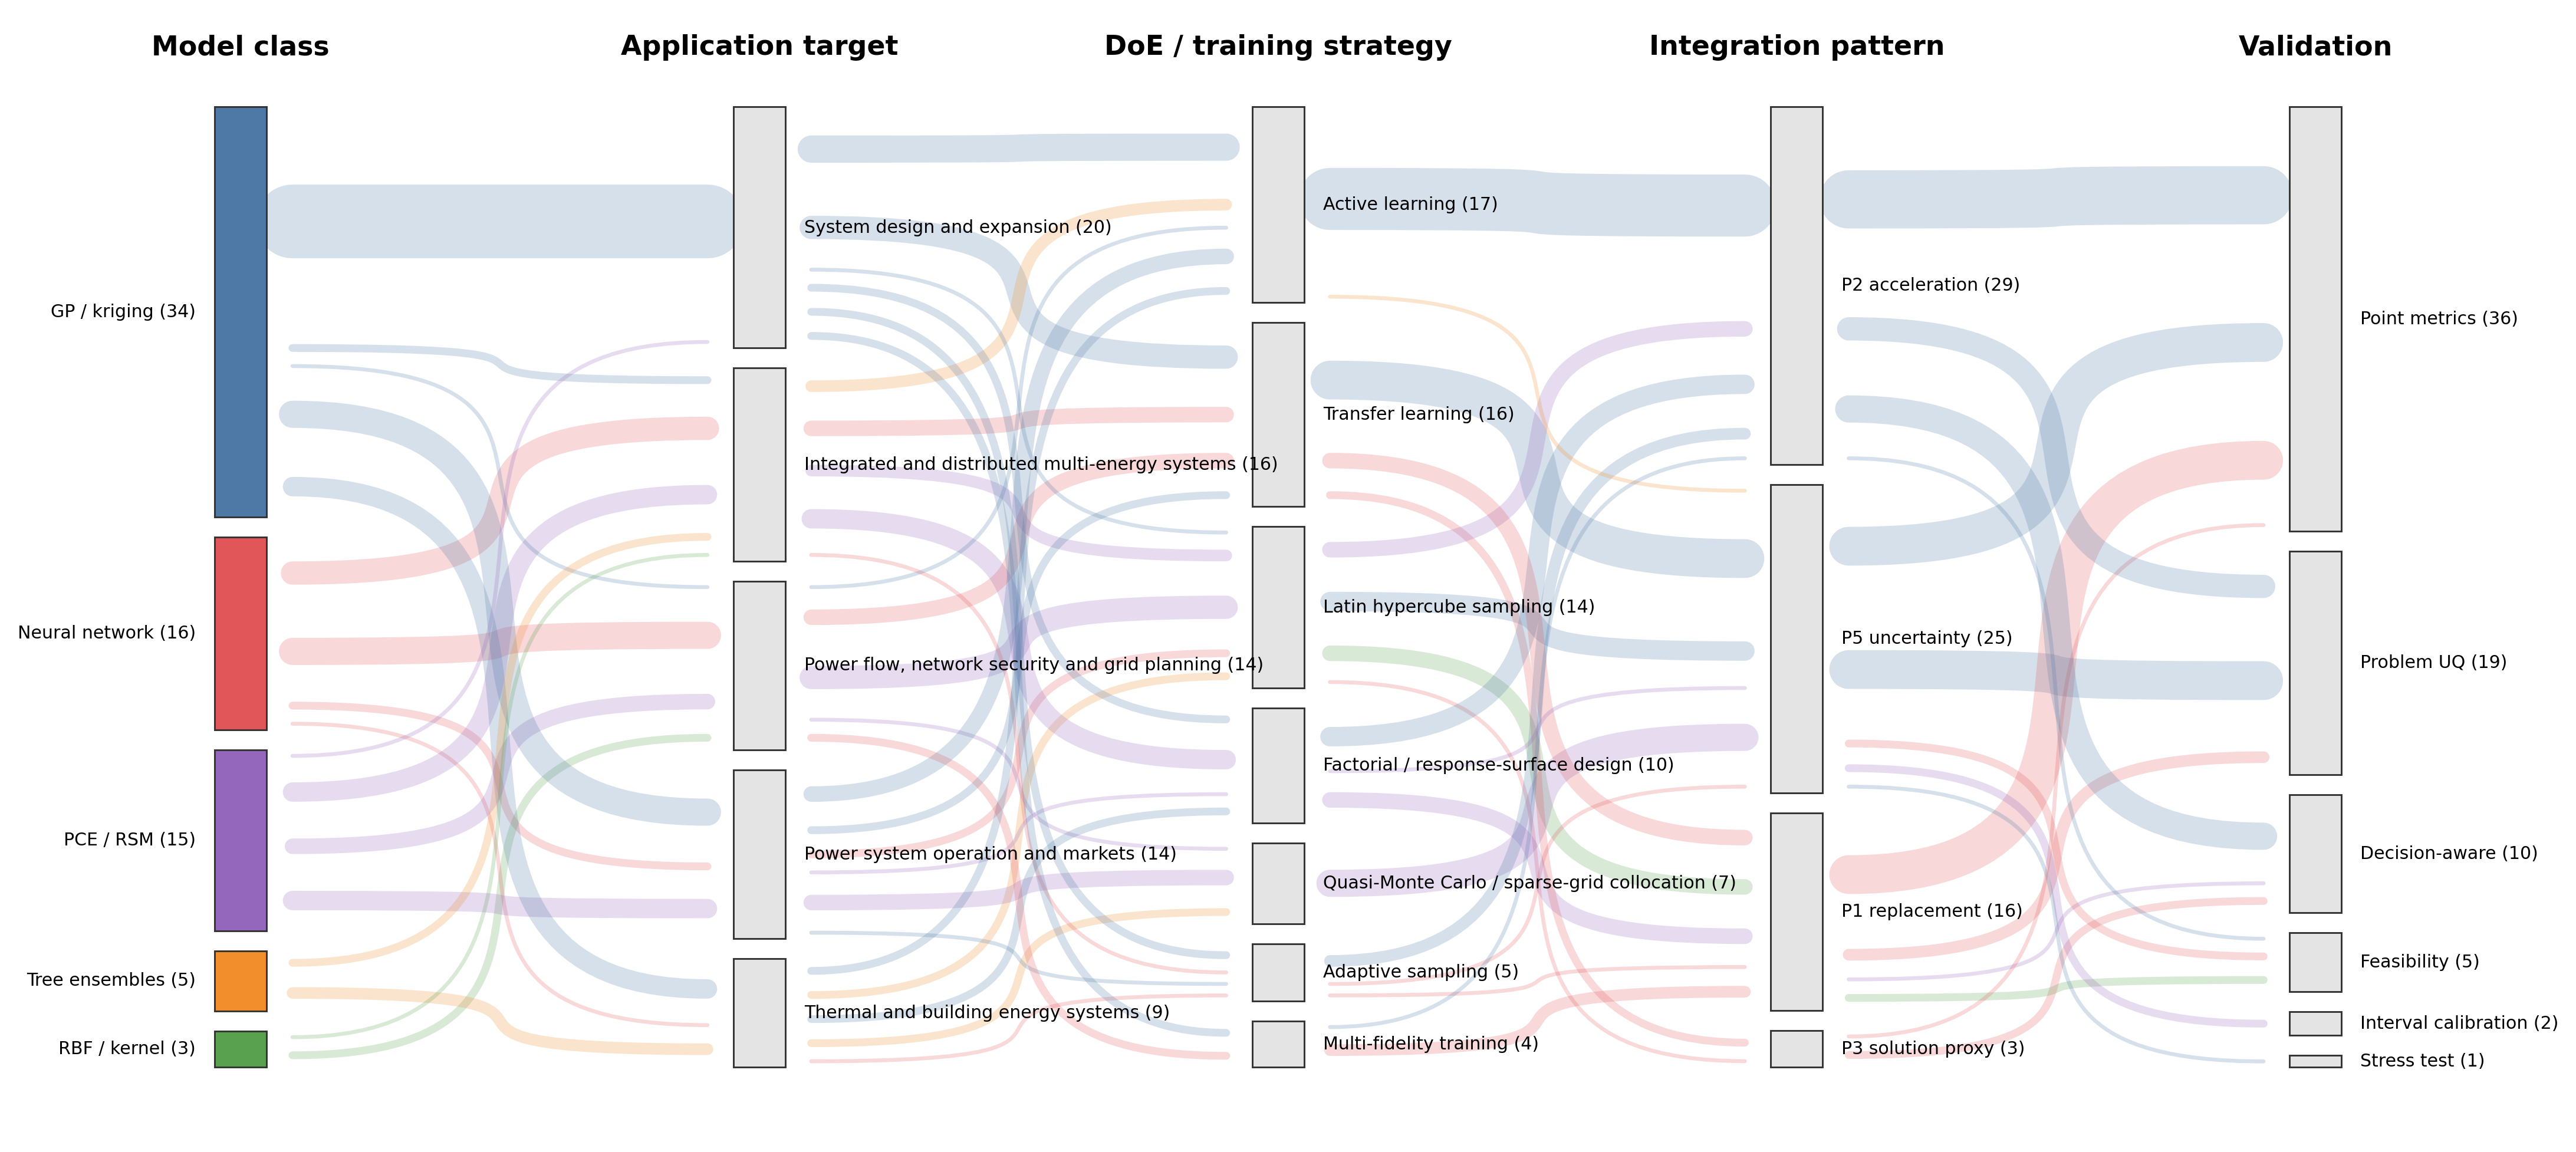
\includegraphics[width=\textwidth]{../figures/fig_taxonomy_alluvial_flow_evidence.png}
\caption{Evidence-based flow from surrogate model class through DoE and training, integration pattern and validation practice. Only studies with explicit assignments across the plotted stages are included.}
\label{fig:evidence-alluvial}
\end{figure*}

FigureÂ~\ref{fig:evidence-alluvial} shows how the methodological
dimensions are connected across the evidence base. FigureÂ~\ref{fig:application-target-taxonomy} then compares model
classes, DoE and training choices, integration patterns and validation
practices across the same five application-target domains. Counts in
the panels refer to explicit study-level category assignments; one study
can contribute to more than one DoE or validation category.

\begin{figure*}[!t]
\centering
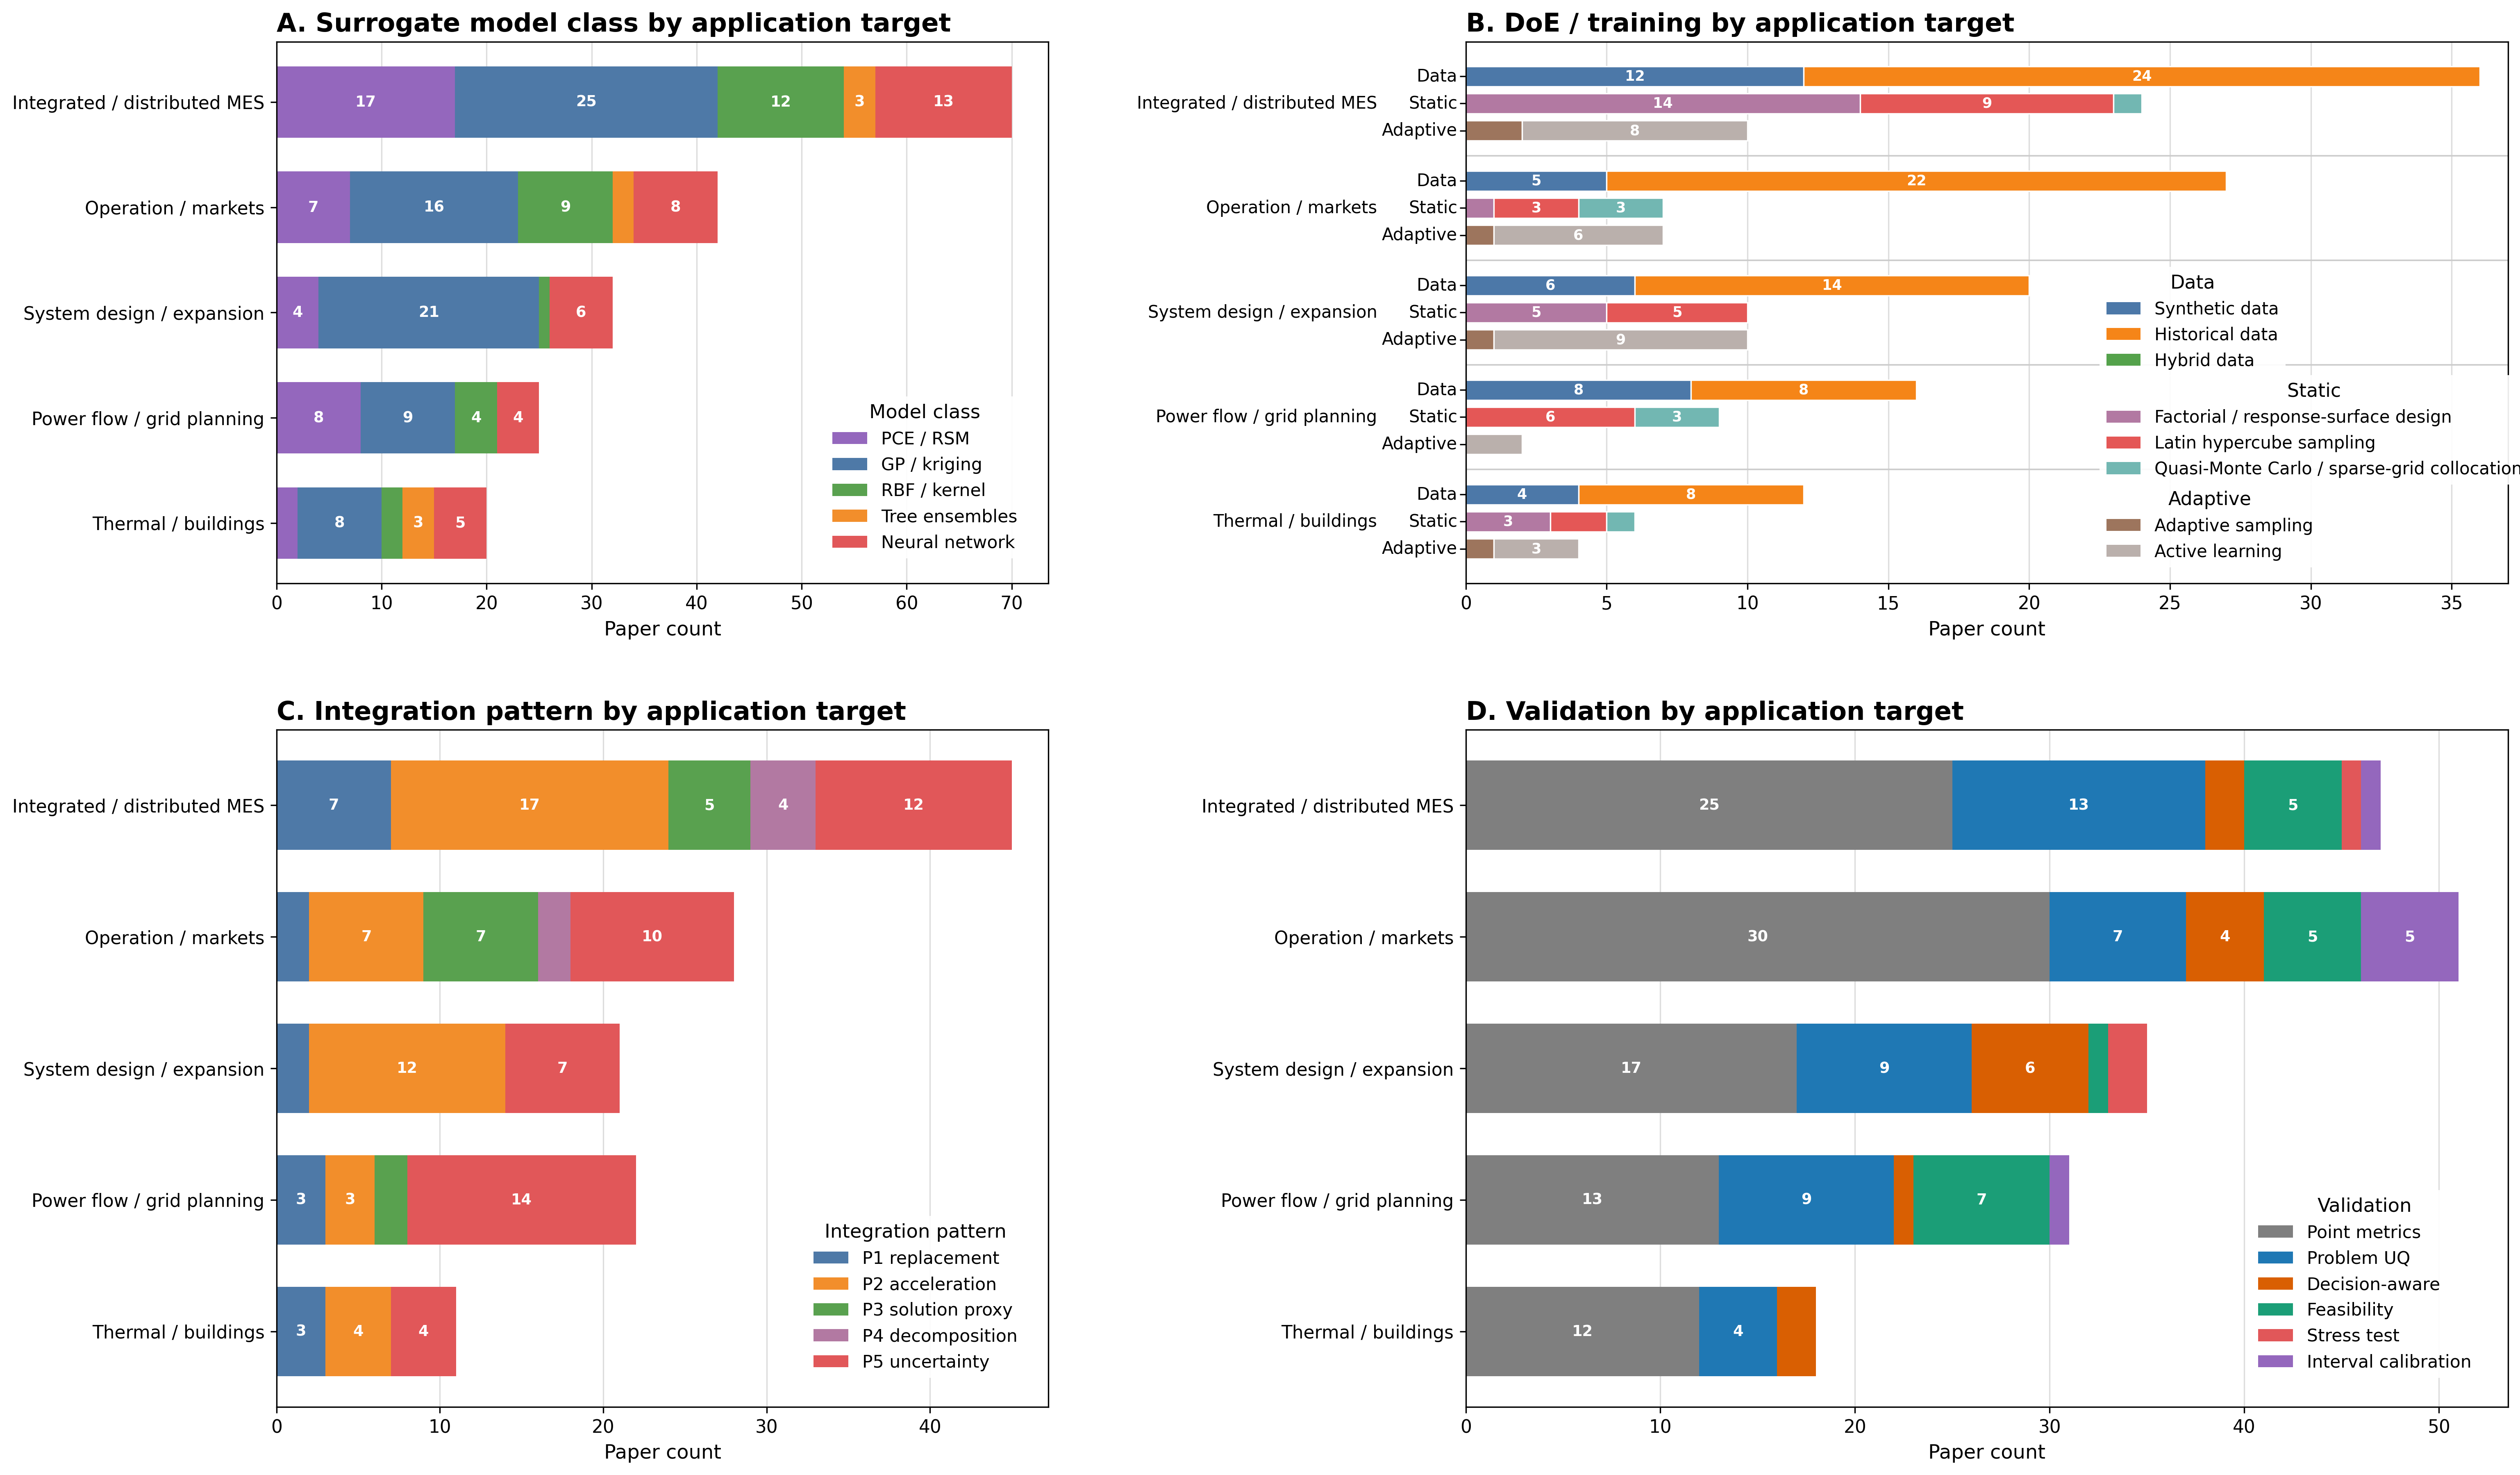
\includegraphics[width=\textwidth]{../figures/fig_four_panel_application_target_taxonomy.png}
\caption{Quantitative evidence by application target. Panels A to D show the surrogate model class, data source and DoE strategy, integration pattern, and validation practice. Counts are based on explicit study-level assignments; unresolved labels are omitted.}
\label{fig:application-target-taxonomy}
\end{figure*}

\subsubsection{Integrated and distributed multi-energy systems: multi-energy and sector-coupled systems}
\label{sec:apps:mes}

MES applications cover electricity--heat--gas coupling, integrated
dispatch and system design. Several studies use surrogates as P1
replacements for repeated inner optimisation solves. Ren et
al.Â~\cite{Ren2024} use a NN-based surrogate for heterogeneous multi-energy
storage deployment and place the training inputs by LHS. Jalving et
al.Â~\cite{Jalving2023} use a NN-based surrogate in conceptual design and
optimisation of integrated energy systems, and Franzoso et
al.Â~\cite{Franzoso2025} use a NN-based surrogate-assisted formulation in the
context of DRL for energy-system analysis and optimisation.

A second group focuses on uncertainty-aware MES operation. Zhou et
al.Â~\cite{Zhou20181} use a GP/kriging surrogate in robust optimisation of an
integrated community energy system and report prediction-interval
calibration. Dong et al.Â~\cite{Dong2022} also use a GP/kriging surrogate for
uncertainty propagation in robust MPC of an RES-CCHP system. Wang et
al.Â~\cite{Wang2020202933} use a PCE/RSM surrogate to replace repeated inner
solves in IES scheduling with scheduling elasticity. Dong et
al.Â~\cite{Dong2023} use a PCE/RSM surrogate for chance-constrained IES
dispatch, with sparse-grid or PCE-collocation sampling and feasibility
or constraint-violation checks. Zheng et al.Â~\cite{Zheng20231907} use a
GP/kriging surrogate for distributed electricity--heat dispatch with
variable mass flow and report feasibility or constraint-violation
validation. Shi et al.Â~\cite{Shi2024__2} use a GP/kriging surrogate in a
decomposition-layer setting for regional IES load forecasting.

\subsubsection{System design and expansion: multi-objective energy system design}
\label{sec:apps:moo}

MOO energy-system design is mainly a P2 application area, because many
candidate designs must be evaluated while approximating a Pareto front.
PCE/RSM surrogates are used inside outer MOO or evolutionary search in
campus multi-energy systems \cite{Dong2024}, solar-integrated trigeneration
systems with structured DoE \cite{Salahinezhad2025}, strategic stochastic
planning with feasibility or constraint-violation validation
\cite{alahmad_enhancing_2025}, and stochastic optimisation of renewable and
green technologies with stress-test validation
\cite{alahmad_optimizing_2025}. The same PCE/RSM pattern is used for
hydrogen systems and demand response with RES and EVs
\cite{ali_optimizing_2025}, shared BESS placement with feasibility or
constraint-violation validation \cite{an_multi-objective_2025}, renewable
planning with an improved Frilled Lizard algorithm
\cite{bendriss_novel_2025}, biomass--solar--wind multi-energy systems with
feasibility or constraint-violation validation
\cite{chen_multi-objective_2025-1}, NSGA-II-based MOO
\cite{cortes-caicedo_multi-objective_2025}, pumped-storage operation
\cite{liang_high_2024}, Power-to-X conversion \cite{malla_sg_optimization_2024},
and green-hydrogen HRES design with factorial training designs
\cite{tezer_multi-objective_2025}.

NN-based surrogates are also used in outer MOO or evolutionary search.
Wang et al.Â~\cite{Wang2024} use a NN surrogate for PV-based hydrogen--oxygen
co-production and report feasibility or constraint-violation validation.
Lalitha et al.Â~\cite{Lalitha20231401} use a NN surrogate in
surrogate-assisted particle swarm optimisation for microgrid protection.
Reis et al.Â~\cite{Reis2025} use a NN surrogate in symmetry-guided
surrogate-assisted NSGA-II, with further simulations selected by
BO-style active learning. Bagheri et al.Â~\cite{bagheri_miqcp-based_2025} use
a NN surrogate in an MIQCP-based MOO operation strategy for
renewables-integrated smart systems. Tian et al.Â~\cite{tian_building_2025}
use a NN surrogate trained from historically observed operating data for
building design and operation MOO and report feasibility or
constraint-violation validation.

Other MOO studies use GP/kriging or RBF-type surrogates. Zhang et
al.Â~\cite{Zhang20234075} use a GP/kriging surrogate for multimodal MOO of an
HRES. Han et al.Â~\cite{Han2018622} use an RBF/kernel surrogate for dynamic
VAR planning with short-term voltage considerations. Not all MOO-related
studies are pure outer-loop search cases: Dong et al.Â~\cite{Dong2023__2} use
a PCE/RSM surrogate to replace inner optimisation solves in robust IES
scheduling, while Abbas et al.Â~\cite{abbas_optimal_2024} use a PCE/RSM
surrogate in a decomposition-layer setting for grid-connected
distributed-resource scheduling and report feasibility or
constraint-violation validation.

\subsubsection{Integrated and distributed multi-energy systems: microgrids and energy hubs}
\label{sec:apps:microgrid}

Microgrid, energy-hub and VPP studies cover controller tuning,
scheduling, sizing, bidding and energy management. Several
controller-tuning papers use PCE/RSM surrogates inside outer MOO or
evolutionary search. Hussien et al.Â~\cite{Hussien20211883} use factorial
designs for PI-control tuning with a sunflower optimisation algorithm.
Hussien et al.Â~\cite{Hussien20226442}, Hussien et al.Â~\cite{Hussien202190577}
and Hussien et al.Â~\cite{Hussien202415075} use discrete-factor
response-surface fitting for PI-control tuning in autonomous or islanded
microgrid operation. Arar Tahir et al.Â~\cite{arar_tahir_scientific_2023} use
LHS for a PCE/RSM surrogate in optimisation of microgrids with renewable
energy systems. Batista et al.Â~\cite{batista_optimizing_2023} use the same
surrogate role for HRES-powered reverse-osmosis plants.

RBF/kernel surrogates are mainly used as P1 replacements for repeated
evaluations in microgrid and energy-hub operation. Faraji et
al.Â~\cite{Faraji2020157284} use an RBF/kernel surrogate for day-ahead
self-scheduling and operation of prosumer microgrids. Wang et
al.Â~\cite{Wang20192635} use an RBF/kernel surrogate trained from
historically observed operating data for power-management optimisation
in a hybrid microgrid. Lu et al.Â~\cite{Lu20232989} use an RBF/kernel
surrogate trained from historical operating data for distributed online
microgrid dispatch and report feasibility or constraint-violation
validation. Wu et al.Â~\cite{Wu2021} use an RBF/kernel surrogate for AA-CAES
energy-hub bidding and scheduling, with further simulations selected by
BO. Zhang et al.Â~\cite{Zhang20203731} use an RBF/kernel surrogate for
two-stage isolated-microgrid operation and transfer information across
related datasets.

GP/kriging and NN surrogates are also common P1 replacements in this
application group. Eseye et al.Â~\cite{Eseye201991463} use a GP/kriging
surrogate for electricity-demand modelling with integrated feature
selection. Rigo-Mariani et al.Â~\cite{Rigo-Mariani20171762} use a GP/kriging
surrogate for integrated smart-microgrid design with storage. Gan et
al.Â~\cite{Gan2021695} use GP forecasting with MPC for an interconnected EMS,
and Kanwal et al.Â~\cite{Kanwal2018117} use SVM and GP regression for
PV-power modelling. Guo et al.Â~\cite{Guo20222057} use a NN surrogate for
optimal power allocation in islanded microgrids. Chaturvedi et
al.Â~\cite{Chaturvedi2024149} use a NN surrogate in RL-based integrated
control of DC microgrids. Roth et al.Â~\cite{Roth2019214} formulate a
modular MILP metamodel architecture for HRES design. Liu et
al.Â~\cite{Liu20242534} use a
hard-constrained NN surrogate for hybrid AC/DC microgrid energy
management.

Uncertainty-aware microgrid and VPP studies mainly follow P5.
Nematollahi et al.Â~\cite{Nematollahi2021} use a GP/kriging surrogate for DER
sizing and siting in active distribution networks. Kiani et
al.Â~\cite{Kiani20253021} use a GP/kriging surrogate for robust MPC in
islanded microgrid voltage control. Han et al.Â~\cite{Han2024} use a
GP/kriging surrogate for hierarchical robust day-ahead VPP--DSO
coordination. Pourmohammadi et al.Â~\cite{Pourmohammadi2023} use a PCE/RSM
surrogate for robust metamodel-based HRES design. Yang et
al.Â~\cite{Yang2024__2} use a PCE/RSM surrogate for robust day-ahead to
intra-day microgrid scheduling and include stress-test validation. Wang
et al.Â~\cite{Wang20211767} use an RBF/kernel surrogate for stochastic
residential demand response with UC and TOU pricing.

Other studies show additional integration roles within microgrid and
energy-hub applications. Kaewdornhan et al.Â~\cite{Kaewdornhan2022130373} use
a NN surrogate in outer MOO or evolutionary search for
distribution-network management with multi-microgrids and report
feasibility or constraint-violation validation. Perera et
al.Â~\cite{Perera2017187} use a NN surrogate for distributed energy-hub
design and select further simulations by active learning. Cao et
al.Â~\cite{Cao2023__2} replace inner solves in VPP co-optimisation with
electricity--heat--carbon trading and use LHS for the training inputs.
Xu et al.Â~\cite{Xu20184696} use a PCE/RSM surrogate to replace inner solves
in islanded-microgrid loadability analysis and represent uncertainty by
sparse-grid or PCE-collocation nodes. Li et al.Â~\cite{Li2023__3} train a
sparse variational GP surrogate on historical data to imitate
electricity and heat-flow calculations for multi-agent energy
management of multiple microgrids. Matta et
al.Â~\cite{Matta2026} use a GP/kriging surrogate with active learning for
near-optimal isolated-microgrid design and report prediction-interval
calibration. Velásquez et al.Â~\cite{velasquez_intelligence_2023} use an
RBF/kernel surrogate inside outer MOO or evolutionary search.

\subsubsection{Thermal and building energy systems: district heating and thermal storage}
\label{sec:apps:dh}

DH and thermal-storage studies are closely related to the modelling
setting discussed earlier, because building or thermal-network models
are often too expensive to embed directly in system-level optimisation.
Hirvonen et al.Â~\cite{Hirvonen2017323} use a NN metamodel in MOO of a
high-latitude solar community and report feasibility or
constraint-violation validation. Sánchez-Zabala et
al.Â~\cite{Sánchez-Zabala2024} compare several machine-learning algorithms
and use boosting-based building metamodels in a district
energy-management optimisation testbed. They report point-prediction
accuracy and validate the models on buildings not used for training.

Further DH-related studies use surrogates either as P1 replacements or
as P5 uncertainty components. Weinberger et al.Â~\cite{Weinberger2018555} use
a NN surrogate for combined heat and power analysis and train it with a
Box--Behnken design. Reich et al.Â~\cite{Reich2020} use a GP/kriging
surrogate for predictive DH control. Chaudhry et al.Â~\cite{Chaudhry2024} use
a PCE/RSM surrogate for robust fifth-generation DHC analysis, with
sparse-grid or PCE-collocation nodes for uncertain inputs. Du et
al.Â~\cite{Du2025} use a NN surrogate to improve energy flexibility of an
integrated system under uncertainty.

\subsubsection{Power-system operation and markets: economic dispatch and unit commitment}
\label{sec:apps:dispatch}

Dispatch and UC studies focus on repeated LP/MILP-type solves, nonconvex
economic dispatch, stochastic dispatch and learning-based proxies. NN
surrogates are often used as P1 replacements for SCUC, SCED and
economic-dispatch evaluations. Wu et al.Â~\cite{Wu2022231} use a NN surrogate
for SCUC with uncertain wind power. Chen et al.Â~\cite{Chen20244723} use a NN
surrogate as an end-to-end feasible optimisation proxy for large-scale
economic dispatch and report regret or optimality-gap checks. Chen et
al.Â~\cite{Chen2022} use a NN surrogate for large-scale SCED and report
feasibility or constraint-violation validation. Xu et al.Â~\cite{Xu20223066}
use an ensemble DNN for nonconvex economic dispatch, and Guo et
al.Â~\cite{Guo202115024} use a learning-based approach for economic dispatch
in smart grids.

PCE/RSM surrogates are mainly used for uncertainty propagation in
stochastic or reliability-constrained dispatch. Safta et
al.Â~\cite{Safta20172535} use PCE/RSM for stochastic economic dispatch,
represent uncertain inputs by sparse-grid or PCE-collocation nodes and
report feasibility or constraint-violation validation. Wang et
al.Â~\cite{Wang2022812}, Li et al.Â~\cite{Li20191438} and Lu et al.Â~\cite{Lu201991827}
also use PCE/RSM with sparse-grid or PCE-collocation nodes for
stochastic economic dispatch under renewable uncertainty. Pan et
al.Â~\cite{Pan20244422} use PCE/RSM for reliability-constrained economic
dispatch, also with sparse-grid or PCE-collocation nodes and feasibility
or constraint-violation validation.

Other dispatch applications use RBF/kernel, PCE/RSM or GP/kriging
surrogates as P1 replacements. Rafi et al.Â~\cite{Rafi202132436} use an
RBF/kernel surrogate in short-term load forecasting with integrated CNN
and LSTM components. Dullinger et al.Â~\cite{Dullinger20181646} use an
RBF/kernel surrogate for MILP-based HVAC predictive control. Goudarzi et
al.Â~\cite{Goudarzi2017667} use an RBF/kernel surrogate for real-time
scheduling of generating units. Ahmad et al.Â~\cite{Ahmad202451} use a
PCE/RSM surrogate for wastewater electrolysis and train it with a
Box--Behnken design. Rixhon et al.Â~\cite{Rixhon2021} use a PCE/RSM surrogate
for electrofuels in the Belgian energy transition, with quasi-Monte
Carlo sampling. Angizeh et al.Â~\cite{Angizeh2023134995} use a GP/kriging
surrogate for grid integration of storage and renewables and report
prediction-interval calibration. Yan et al.Â~\cite{Yan2019625} use a
GP/kriging surrogate for wind-generation interval forecasts and also
report prediction-interval calibration.

GP/kriging also appears in search and uncertainty settings. Nikolaidis
et al.Â~\cite{Nikolaidis2021} use GP-based BO for data-driven UC, where
further simulations are chosen by acquisition-driven active learning.
Lin et al.Â~\cite{Lin2023} use a GP/kriging surrogate in a search-loop
formulation for combined economic/emission dispatch. Hu et
al.Â~\cite{Hu2021671} use GP/kriging for uncertainty propagation in
stochastic economic dispatch, with sparse-grid or PCE-collocation nodes.
Hu et al.Â~\cite{Hu2020} use GP emulation for stochastic economic dispatch
and place training inputs by LHS. Further dispatch and UC examples
include deep neural networks embedded in Surrogate Lagrangian
Relaxation for UC \cite{Wu2024391}, a NN surrogate inside an
adaptive bat algorithm for large-scale economic dispatch \cite{Pang2023},
and a constraint-aware neural surrogate for joint chance-constrained UC
\cite{Liang20246508}.

\subsubsection{Power flow, network security and grid planning: optimal power flow and AC relaxations}
\label{sec:apps:opf}

OPF work mainly uses surrogates to approximate nonlinear AC-OPF or
load-flow evaluations, or to propagate uncertainty in chance-constrained
and robust formulations. PCE/RSM surrogates are used for
chance-constrained AC-OPF by Muhlpfordt et al.Â~\cite{Muhlpfordt20194806}, PV
hosting-capacity calculation by Koirala et al.Â~\cite{Koirala20242284}, OPF
with non-Gaussian uncertainties by Muhlpfordt et
al.Â~\cite{Muhlpfordt20174490}, iterative response-surface chance-constrained
AC-OPF by Xu et al.Â~\cite{Xu20212696}, and current--voltage OPF by Van Acker
et al.Â~\cite{Van Acker2022}. These PCE/RSM studies use sparse-grid or
PCE-collocation nodes for uncertain inputs, and Xu et al.Â~\cite{Xu20212696}
and Van Acker et al.Â~\cite{Van Acker2022} report feasibility or
constraint-violation validation.

RBF/kernel surrogates are used as P1 replacements in reliability,
stability, prediction and TCSC-allocation problems. Urgun et
al.Â~\cite{Urgun20202791} use an RBF/kernel surrogate for
composite-power-system reliability and place training inputs by LHS. Liu
et al.Â~\cite{Liu20223726} use an RBF/kernel surrogate for
small-signal-stability-constrained OPF. Wu et al.Â~\cite{Wu2021__2} use an
RBF/kernel surrogate for short-term power prediction with an improved
bird swarm algorithm. Mahapatra et al.Â~\cite{Mahapatra20161921} and
Mahapatra et al.Â~\cite{Mahapatra2022721} use RBF/kernel surrogates for TCSC
location, sizing or allocation in OPF-related settings.

GP/kriging surrogates are used both for OPF replacement and
chance-constrained OPF. Deng et al.Â~\cite{Deng2020831} use kriging-assisted
surrogate evolutionary computation for OPF and add training points
sequentially by infill rules. Mitrovic et al.Â~\cite{Mitrovic2023__2} use
hybrid sparse GPs for data-driven chance-constrained AC-OPF and report
feasibility or constraint-violation validation. Mitrovic et
al.Â~\cite{Mitrovic2023__3} use GP-based chance-constrained OPF in a
software-tool setting. Katkar et al.Â~\cite{Katkar2025} use GP/kriging in an
ensemble surrogate archive-assisted metaheuristic for OPF-related
multi-modal optimisation.

Distribution-network planning and stochastic OPF studies also use
uncertainty-focused surrogates. Fu et al.Â~\cite{Fu20202904} use PCE/RSM for
stochastic distribution-network planning and train with LHS. Fu et
al.Â~\cite{Fu2022} use PCE/RSM for capacitor planning under PV uncertainty,
with discrete-factor response-surface fitting and feasibility or
constraint-violation validation. Engelmann et al.Â~\cite{Engelmann20186188}
use PCE/RSM for distributed stochastic AC-OPF, with sparse-grid or
PCE-collocation nodes and feasibility or constraint-violation
validation. Zhang et al.Â~\cite{Zhang2024821} use GP/kriging for
distributionally robust chance-constrained conservation voltage
reduction, and Liu et al.Â~\cite{Liu20222679} use GP/kriging for data-driven
probabilistic load-flow studies.

NN, constraint-aware NN and tree-ensemble surrogates appear in fast
control and OPF proxy formulations. Su et al.Â~\cite{Su2022315} use a NN
surrogate for fast preventive control and place training inputs by LHS.
Li et al.Â~\cite{Li202359995} use a NN surrogate for optimisation with hard
linear constraints, transfer information across related datasets and
report feasibility or constraint-violation validation. Chen et
al.Â~\cite{Chen2023657} use a constraint-aware neural surrogate for joint
chance-constrained OPF and report feasibility or constraint-violation
validation. Lei et al.Â~\cite{Lei20247417} use a constraint-aware neural
surrogate for chance-constrained DC-OPF with affine control policy and
report feasibility or constraint-violation validation. Srithapon et
al.Â~\cite{Srithapon202134395} use a NN surrogate inside outer MOO or
evolutionary search for probabilistic OPF in distribution networks. Li
et al.Â~\cite{Li2023__2} use neural networks with gauge mappings to
accelerate ADMM-based DC-OPF while enforcing local constraints.

\subsubsection{System design and expansion: capacity and generation expansion planning}
\label{sec:apps:expansion}

Expansion planning re-evaluates operational sub-models across investment
candidates. Park et al.Â~\cite{Park2019} use a NN surrogate in an outer
search-loop setting for physics-induced graph-neural-network wind-farm
power estimation. Jahangiri et al.Â~\cite{Jahangiri20244849} use a NN
surrogate for Canadian provincial power-system decarbonisation analysis,
and Jahangiri et al.Â~\cite{Jahangiri2023} use a NN surrogate-assisted
formulation to explore the Canadian decarbonisation design space.

Uncertainty-aware expansion studies mainly use GP/kriging. Kim et
al.Â~\cite{Kim2021} use a GP/kriging surrogate for probabilistic
wind-energy-potential modelling in power-grid expansion planning. Lawson
et al.Â~\cite{Lawson201647} use a GP/kriging surrogate in a Bayesian
framework for power-network planning under uncertainty. Volodina et
al.Â~\cite{Volodina2022} use a GP/kriging surrogate for uncertainty
propagation in a network of energy models, with LHS training inputs and
prediction-interval calibration.

Other expansion-planning examples use different model classes and roles.
Rodgers et al.Â~\cite{Rodgers2018951} use a PCE/RSM surrogate inside outer
MOO or evolutionary search for generation expansion planning with health
and societal damages. Pérez-Uresti et al.Â~\cite{Pérez-Uresti2023} use a NN
surrogate to replace expensive inner optimisation solves in strategic
hydrogen-economy investment planning. Yang et al.Â~\cite{Yang2025} use a
tree-ensemble surrogate inside adaptive multi-objective BO for
interconnected capacity planning, with further simulations selected by
acquisition-driven active learning.

\subsection{Synthesis: where surrogates help, where they do not}
\label{sec:apps:synthesis}

Taken together, the evidence map supports four observations. *First*,
the five domains differ more clearly by integration role than by model
class. Panel A of
FigureÂ~\ref{fig:application-target-taxonomy} shows GP/kriging as the
largest model-class category in every domain, although PCE/RSM,
RBF/kernel and neural models remain substantial in specific
applications. *Second*, Panel C shows that P2 acceleration is the
largest integration category in integrated and distributed MES. P5
uncertainty is largest in system design and expansion, power flow and
grid planning, and power-system operation and markets. Thermal and
building applications are split more evenly between P1 replacement, P2
acceleration and P5 uncertainty. These
domain-level patterns are consistent with the cross-dimensional flows
in FigureÂ~\ref{fig:evidence-alluvial}. *Third*, Panel B shows that
historical data form the largest recorded data-source category in all
five domains, although in power flow and grid planning the historical
count is tied with Latin-hypercube sampling when data-source and DoE
categories are viewed together.
*Fourth*, Panel D confirms that point metrics dominate validation in all
five domains. Problem-level uncertainty is the next most frequent
category, while feasibility, stress testing, interval calibration and
decision-aware evaluation remain less common. For integrated MES and
system-design applications, an open issue therefore remains how
surrogate-derived Pareto or robust solutions should be validated and
communicated to decision makers
\cite{Mylonopoulos202332697,Lim2025}.

\section{Software-packages in surrogate modeling and multi-energy systems}
\label{sec:software}

This section reports only software mentions that were found in the review PDFs
scanned by \texttt{paper\_library/verify\_T8\_software\_cites.py}. The table is
therefore a conservative mention map, not a feature comparison, package
recommendation, maintenance audit, or proof that a package was used in the
primary studies. Packages without a review-PDF mention are omitted, even if
they are widely used in practice.

\begin{table*}[!t]
\centering
\scriptsize
\caption{Software packages and environments explicitly mentioned in the review PDFs scanned for this paper. The table records mention evidence only; it does not claim package maintenance status, GPU support, license, or built-in surrogate--MES integration.}
\label{tab:T8-software-packages}
\renewcommand{\arraystretch}{1.10}
\begin{tabularx}{\textwidth}{@{}L{0.20\textwidth} L{0.18\textwidth} L{0.34\textwidth} L{0.20\textwidth}@{}}
\toprule
Package / environment & Software block & Conservative use/context from review-PDF mentions & PDF-screen evidence \\
\midrule
\texttt{ALAMO}; \texttt{Eureqa}; Surrogates Toolbox; \texttt{SUMO}; \texttt{ARGONAUT}; \texttt{scikit-learn}; R-side packages &
Surrogate / ML software &
Surrogate modelling, validation, derivative-free optimization, and general ML regression in the surrogate-methodology review context. &
Bhosekar et al. mention these packages and toolboxes \cite{Bhosekar2018}. \\
\texttt{GPML}; \texttt{GPy}; \texttt{GPflow}; \texttt{GPyTorch}; \texttt{BoTorch}; \texttt{PyMC3}; \texttt{Pyro} &
GP / probabilistic software &
Gaussian-process modelling, probabilistic programming, and Bayesian-optimization-related tooling in a GP-for-power-systems review context. &
Tan et al. mention these GP and probabilistic software packages \cite{Tan2026}. \\
\texttt{XGBoost}; \texttt{LightGBM}; \texttt{TensorFlow}; \texttt{PyTorch}; \texttt{MATLAB} &
ML / engineering environments &
Learning-assisted power-system models, building-energy or HRES surrogate contexts, digital-twin workflows, and general engineering optimization environments, depending on the review. &
PDF-screen mentions in learning-assisted power, surrogate, digital-twin, building-energy and HRES reviews \cite{Khaloie2025,Conti2026,Zhang2026_building,Lim2025,Elwy2024,Tan2026,FernandezGodino2023,Westermann2019,Li2025_hydrogen,Etghani2025}. \\
\texttt{SMT} &
Surrogate toolbox &
Surrogate-modelling toolbox mentioned in energy-related surrogate or digital-twin review contexts. &
PDF-screen mentions in Westermann et al. and Khan et al. \cite{Westermann2019,Khan2024_DT}. \\
\texttt{GAMS}; \texttt{Gurobi}; \texttt{CPLEX}; \texttt{Mosek}; \texttt{IPOPT}; \texttt{BARON} &
Modelling language / solvers &
Algebraic modelling and mathematical optimization backends in ESM, MES, power-system learning, or surrogate-optimization review contexts. This does not imply a surrogate-specific interface. &
PDF-screen mentions in ESM, MES, power-system learning and surrogate-methodology reviews \cite{Fattahi2020,Klemm2021,Manco2024,Lim2025,Khaloie2025,Westermann2019,Bhosekar2018,Mylonopoulos202332697}. \\
\texttt{PyPSA}; \texttt{oemof}; \texttt{Calliope}; \texttt{OSeMOSYS}; \texttt{TIMES}; \texttt{MARKAL}; \texttt{REMix} &
Energy-system modelling tools &
MES, district-scale, national, or long-term energy-system modelling frameworks discussed as host modelling tools. The screen does not show native surrogate interfaces. &
PDF-screen mentions in MES and national/long-term ESM reviews \cite{Klemm2021,Fattahi2020,ChenRenZhou2023}. \\
\texttt{HOMER}; \texttt{iHOGA}; \texttt{RETScreen} &
Microgrid / HRES tools &
Microgrid, hybrid-renewable-system, ship-energy, hydrogen, or broader energy-system assessment and optimization contexts. &
PDF-screen mentions in microgrid, HRES, hydrogen and broader energy-review PDFs \cite{agha_kassab_comprehensive_2024,Mylonopoulos202332697,nallolla_multi-objective_2023,velasquez_intelligence_2023,arar_tahir_scientific_2023,batista_optimizing_2023,Klemm2021,Li2025_hydrogen,ChenRenZhou2023}. \\
\texttt{EnergyPlus}; \texttt{TRNSYS}; \texttt{Modelica/Dymola} &
Simulation environments &
Building-energy, transient HVAC/renewable-system, thermal-system or multi-physics simulation contexts that can act as high-fidelity models in surrogate workflows. &
PDF-screen mentions in building-surrogate, MES-tool, HRES and thermal-system review PDFs \cite{Westermann2019,Klemm2021,Zhang2026_building,Elsheikh2019622,batista_optimizing_2023,Li2025_hydrogen,Etghani2025,Elwy2024}. \\
\bottomrule
\end{tabularx}
\end{table*}

Two cautious observations follow from this evidence. First, the review-level
software evidence is fragmented: surrogate-methodology reviews discuss
surrogate and GP software, whereas MES and HRES reviews mostly discuss
modelling environments, simulators and optimization solvers. Second, the
scanned reviews do not provide enough evidence to claim a mature,
standardized interface between surrogate libraries, multi-objective decision
workflows and energy-system modelling tools. For this reason, the open
challenge is not that a specific package is missing, but that
review-documented evidence for reproducible surrogate--MES toolchain
integration remains limited.

\section{Open challenges and research directions}
\label{sec:challenges}
The evidence map and the section-level synthesis point to six recurring
weaknesses in the current literature. These weaknesses cut across model
classes, integration patterns and application domains. They are not
about whether surrogate models can be useful; they concern how studies
are assembled, validated, compared and reported. The following
subsections focus on those gaps that appear repeatedly and that are most
relevant for future surrogate-assisted MES work.
\subsection{Decision-aware benchmarking}
\label{sec:ch:bench}
The most immediate gap is the lack of decision-aware benchmarks.
Predictive metrics are reported in many studies, but direct evidence on
decision quality is often limited to a few example runs. Speed-up claims
are common; regret distributions, feasibility rates and worst-case
violations are much rarer
\cite{Mylonopoulos202332697,Ruan2021221,Khaloie2025,Lim2025,Perera2019191}.
This makes it difficult to compare methods across papers, even when they
address similar tasks. A useful benchmark would fix the host problem,
the training set, the stress-test set and the solver-time budget, and
would require all methods to report the same decision-oriented outputs:
regret, feasibility rate, MIP-gap distribution, violation severity and
wall-clock savings. Recent learning-to-optimize work for
security-constrained dispatch and unit commitment shows that these
metrics can be reported in a systematic way
\cite{Wu2022231,Chen20244723,Chen2022,Wu2024391,Liang20246508}, but
the field still lacks a shared benchmark that would make results
directly comparable.
\subsection{Calibrated uncertainty for surrogate-assisted MOO}
\label{sec:ch:uq}
Uncertainty handling remains uneven. In surrogate-assisted MOO and in
chance-constrained formulations, the optimization logic depends on
posterior uncertainty, not only on the mean prediction. Yet calibration
is checked much less often than pointwise fit, and several studies
report breakdown precisely in those operating regions that are weakly
covered by the training set
\cite{Hu2020,Hu2021671,Volodina2022,Lawson201647,Hu2024,Buchanan2024,Subedi2026157}.
The field already has practical tools such as deep ensembles, Bayesian
last layers, conformal prediction and polynomial-chaos-based chance
constraints
\cite{Chen2023657,Liang20246508,Muhlpfordt20194806,Koirala20242284,Xu20212696}.
The unresolved issue is how to combine these tools with surrogate-
assisted search and uncertainty-constrained optimization so that the
reported uncertainty still reflects what the optimizer sees at the
relevant points in the design or operating space.
\subsection{Out-of-distribution generalisation across capacity mixes}
\label{sec:ch:ood}
Planning studies use surrogates to say something about systems that do
not yet exist in their final form. This means that the relevant test is
often out-of-distribution by construction: another capacity mix, another
weather year, another operating regime, or another policy setting. Many
surrogates, however, are trained on historical operation or on samples
generated from a much narrower design space
\cite{Park2019,Reynolds2017704,Subedi2026157,Khaloie2025,Lim2025,Mylonopoulos202332697}.
Two practical responses appear in the literature. One is to build more
physics-aware surrogates that preserve balances, monotonicity or other
structural constraints
\cite{Park2019,Su2022315,Liu20223726,Petrova2025,Du2025}. The other
is to fine-tune a base surrogate with a small number of new
high-fidelity runs when climate, year or capacity mix changes
\cite{Chen202514792,De Castro20247710}. What is
still missing is a common way of reporting this distinction, so that
within-distribution accuracy is not confused with planning-relevant
robustness.
\subsection{Standardised public datasets and reproducibility}
\label{sec:ch:data}
The reproducibility audit in Section 8.6 showed a familiar pattern:
many studies describe the case study and the model idea, but not the
full artefacts needed to reproduce the result. Our evidence audit found
few public datasets, especially for district heating, sector-coupled MES
and other settings in which surrogate-assisted optimization would be
most useful.
The bulk of MES surrogate work is still built around individual case
studies. A useful minimum standard would be a public optimization
instance, the corresponding training data, an explicit train/validation/
test split, solver settings and a small number of reference truth-model
runs. Existing load and renewable forecasting datasets
\cite{Eseye201991463,Faraji2020157284,Hanifi2024,Sideratos2020,Tian2020,Madhukumar20228891}
show that this level of release is feasible.
\subsection{MCDM under surrogate uncertainty}
\label{sec:ch:mcdm}
The literature on multi-criteria decision making after surrogate-
assisted MOO is still thin, although this is exactly the step at which a
planner or designer needs a final decision. Some studies combine
response-surface MOO with a subsequent multi-criteria selection
\cite{Roy2020}, but the reviewed literature rarely propagates surrogate
uncertainty into that final ranking. In most multi-objective studies,
the Pareto set is presented and a compromise design is selected without
quantifying whether surrogate error could change the ordering.
For MES planning, this is a concrete gap: uncertainty should not stop at
the Pareto front but should be carried through to the final ranking or
selection step.
\subsection{Open-source libraries and toolchain integration}
\label{sec:ch:tooling}
The final gap is practical rather than conceptual. Several strands of
the literature already have working toolchains -- for example
polynomial-chaos OPF, learning-to-optimize for dispatch, or surrogate-
assisted evolutionary design -- but each strand tends to build its own
data pipeline, evaluation logic and reporting format
\cite{Muhlpfordt20194806,Mitrovic2023__2,Mitrovic2023__3,Wu2022231,Chen20244723,Chen2022,Hirvonen2017323,Schulte2020}.
This fragmentation makes reuse difficult and slows down comparison
across model classes and applications. A shared open-source layer would
not need to replace existing host optimizers; it would be enough to
standardize surrogate input/output interfaces, validation routines and
reporting formats. Frameworks such as PyPSA, Calliope, oemof, SpineOpt
and Backbone already provide a basis on the optimization side. The
surrogate side is still scattered.

\section{Conclusion}
\label{sec:conclusion}
This review set out to examine surrogate-assisted energy system
optimization with a particular focus on multi-energy systems and
multi-objective settings. The main result is not a single best model
class, but a clearer picture of how the field is structured. Model class
alone is not enough to explain the literature. The same Gaussian
process, neural network or polynomial surrogate can serve different
purposes depending on what it approximates, where it is inserted into
the optimization workflow, and how its output is validated. For that
reason, the review organized the field along four linked dimensions:
model class, surrogate target, integration depth and trust mechanism.
This was complemented by a synthesis of training-data generation,
design-of-experiments choices, integration patterns, validation
practice, and application evidence.
Three observations stand out across the reviewed studies. First,
surrogates are already used in several distinct ways rather than in one
generic pattern. Some studies replace expensive inner evaluations,
others accelerate search, provide warm starts, support decomposition, or
handle uncertainty. The dominant pattern depends on the underlying
decision problem. Second, substantial computational savings are reported
across many applications, but the supporting evidence is uneven. Runtime
reductions are usually shown more clearly than their effect on decision
quality. Third, the most active application area is multi-objective
design in microgrids, hybrid renewable systems and broader MES
configurations, while stronger validation practice is more common in
dispatch, unit commitment and OPF studies.
The evidence map also shows where the field is still thin. Publicly
reusable datasets are scarce, especially for district heating and
sector-coupled MES cases. Validation is often still centered on
predictive fit rather than on feasibility, regret or ranking stability.
Many studies mix surrogate modeling, optimization and domain
engineering effectively at case-study level, but the reporting style
does not yet make those studies easy to compare or reuse. This is where
the six challenge areas discussed above become important: common
benchmarks, calibrated uncertainty, better handling of distribution
shift, reproducible datasets, explicit treatment of uncertainty in MCDM,
and less fragmented toolchains.
Taken together, the review provides a structured and quantitative
overview of surrogate-assisted energy system optimization. It contributes
a taxonomy for organizing the literature, an evidence map for tracing
connections between methods and applications, and a more concrete basis
for discussing where surrogate models already work well and where the
current evidence is still weak. If the field moves toward clearer
benchmarks, better reporting and more reusable case-study artefacts,
surrogate-assisted optimization can become easier to compare, easier to
reproduce and more useful for practical MES decision support.


\bibliographystyle{elsarticle-num}
\bibliography{review_paper_library}
\end{document}
